\documentclass[draft]{agujournal2019}

\usepackage[T1]{fontenc}
\usepackage[utf8]{inputenc}
\usepackage{textcomp}
\usepackage{url}
\usepackage{lineno}
\usepackage{amsmath}
\usepackage{amssymb}
\usepackage{graphicx}
\usepackage{booktabs}
\usepackage{array}
\usepackage{eurosym}
\usepackage{calc}
\usepackage[inline]{trackchanges}
\usepackage{soul}
\usepackage{placeins}
\usepackage{float}
\usepackage{caption}
\usepackage{multirow}
\usepackage{longtable}
\usepackage{colortbl}
\usepackage{tabularx}

\definecolor{tblhead}{HTML}{D9D9D9}
\definecolor{tblsub}{HTML}{F4F4F4}
\definecolor{tblgrid}{HTML}{808080}

% Uncomment for review
% \linenumbers

\journalname{Space Weather}

\begin{document}

\title{Assessment of Geomagnetic Storm Impacts in Virginia: Grid Vulnerability, Economic Consequences, and Mitigation Informed by Data}

\authors{
    Vedaang~Verma$^{1}$,
    Dennies~K.~Bor$^{1}$,
    Edward~J.~Oughton$^{1\ast}$ \\
    \small$^{1}$Department of Geography and Geoinformation Science,
    George Mason University, Fairfax, VA, USA. \\
    \small$^\ast$Corresponding author (email: eoughton@gmu.edu).
}

\begin{abstract}
Geomagnetically induced currents (GICs) pose a major threat to power grid infrastructure, yet current risk assessments
are inadequate for regional analysis that can inform targeted mitigation. The Coupled Space Weather Impact Model (C-
SWIM) presents a novel end-to-end pipeline that maps geomagnetic storm scenarios to power grid and economic
impact. This paper presents the first state-level adaptation of C-SWIM for the state of Virginia to identify major risks in
the power grid and their economic ramifications at a regional level, yielding actionable findings for future mitigation.
The extra-high voltage (EHV) network model for the Virginia + PJM interconnection region was constructed and used for
GIC simulations of 92 historical storms. The results identified the Virginia substations with the greatest risk of failure
under varying storm scenarios. The pipeline concluded with economic analysis, in which Ghosh and Leontief models
were used to assess consumption and production disruption: a 100-year storm is projected to cost Virginia
\$145.5M/day, rising to \$230.6M/day under a 250-year event. Based on the results of the adapted Virginia pipeline, a data-driven method of protective islanding was evaluated for mitigation. This solution protects at-risk or highly important regions of the power grid by disconnecting them from the surrounding network. Cost-benefit analysis over the results of three different island selection algorithms showed that islanding can be economically advantageous for the state of Virginia in nearly all tested storm scenarios, reaching benefit-cost ratios of several thousand to one, but only when both network-wide redistribution and storm directionality are accounted for. 
\end{abstract}
\clearpage
\section{Introduction}

Coronal mass ejections (CMEs), or superheated, electrically conductive plasma expelled from the Sun, can cause geomagnetic storms when directed at Earth. These geomagnetic storms disturb Earth's magnetic field, and their impact depends on the underlying geology and power grid infrastructure \cite{Love2024}.

Specifically, these storms drive geomagnetically induced currents (GICs), quasi-direct current that enters the power grid through grounded transformer neutrals. GICs cause extra-high-voltage (EHV) transformer failure due to thermal saturation, leading to power outages and costly infrastructure damage. These occurrences cascade into critical economic disruption: modeling of extreme space weather in the United States estimates daily losses of \$6.2–41.5 billion across blackout scenarios, with manufacturing, government, and finance the most heavily affected sectors, and more than half the total cost falling outside the blackout zone through supply-chain linkages \cite{Oughton2017}.

But the issue is not just prevalent in theory and modeling; it is grounded in history. The March 1989 storm, seen as the archetypal geomagnetic disturbance, collapsed the Hydro-Québec grid within ninety seconds and left over six million people without power for nine hours or more \cite{Boteler2019}. The largest geomagnetic storm in recorded history predates the modern grid entirely: the 1859 Carrington storm disrupted telegraph networks worldwide as operators reported sparking equipment \cite{Boteler2006}. A storm of this magnitude hitting the current highly interconnected EHV power grid would likely have consequences several times greater than those of recent storms. As such, historical occurrences necessitate worst-case modeling of geomagnetic storms. 

Despite advancements in the analysis of space weather and power grid infrastructure, there is a noticeable disconnect in the study of grid vulnerability and socioeconomic consequences, which are typically analyzed separately \cite{Oughton2019}. This presents an issue as operators of critical infrastructure and policymakers require actionable data such as population impacted and sector-by-sector economic losses to inform mitigation strategies. In other words, a bridge between the physics dimension of the hazard and the socioeconomic implications is imperative for data-driven responses to future geomagnetic storm scenarios. 

The Coupled Space Weather Impact Model (C-SWIM) presents a novel end-to-end pipeline that resolves this issue, using historical storm data to inform a pipeline that measures grid vulnerability and translates those measurements to supply- and consumption-driven socioeconomic ramifications \cite{oughton2026majorspaceweatherrisks}.

Critically, the C-SWIM pipeline runs on a national scale for the United States. While national assessment is important, it also presents limitations as decision-makers such as transmission operators and state energy offices operate at a state level, not a national scale. For data-driven mitigation to truly be realized, regional figures of economic and population impact need to be derived from storm modeling, including specific at-risk substations and regions.

Compounding this gap is a need for the implementation of data-driven mitigation in realistic scenarios. Algorithmic GIC mitigation is a widely studied area: a substantial engineering literature demonstrates how to reduce GIC through corrective control of blocking device placement and transmission line switching \cite{Kazerooni2019}. However, current studies have two key limitations. Firstly, mitigation methods are typically evaluated as optimization problems minimizing engineering objectives such as load shedding or reactive-power violations. This means that the real-world objectives of minimizing economic loss and population affected are not considered when evaluating solutions. Many mitigation strategies are justified by engineering as opposed to the factors decision-makers weigh. Secondly, many mitigation methods are tested on synthetic, small-scale test grids unlike real-world, complex networks. In actual power grids, intervention such as blocking and switching at any local area can cause unwanted side effects, making local heuristics unreliable \cite{Schachinger2023}. Mitigation must be decided based on socioeconomic factors and tested via network-wide analysis on a realistic power grid. 

This paper attempts to resolve the aforementioned gaps by presenting the first regional adaptation of the C-SWIM pipeline for Virginia and a data-driven mitigation method of strategic islanding, justified by cost-benefit analysis. This work's contribution is three-fold: (i) a replicable framework for adapting the physics-engineering-economic pipeline of C-SWIM for any local network, producing regional grid vulnerability and economic losses; (ii) actionable findings of geomagnetic storm risk assessment for Virginia; and (iii) a proposed method of data-driven, protective islanding through a criticality-driven selection heuristic to determine the island and cost-benefit analysis to evaluate the solution.
\clearpage

\section{Literature Review}\label{sec:litreview}

This literature review summarizes the current state of peer-reviewed literature on geomagnetic storms, from the physics of GICs to the socioeconomic consequences to mitigation strategies. The literature review was used to justify the materials and methods tested in building a Virginia-level pipeline and developing data-driven solutions. It also helped determine which elements of the national C-SWIM pipeline presented in \citeA{oughton2026majorspaceweatherrisks} to directly transfer or modify for the regional adaptation. 

\subsection{GIC physics and transformer vulnerability}

The modeling of GICs rests on a canonical framework consolidated by \citeA{BotelerGIC}. Geomagnetic storms cause rapid variations in Earth's magnetic field; by electromagnetic induction, this leads to a geoelectric field at Earth's surface. The strength of this field is determined by geology, with more resistive rock leading to greater strength. While this field is induced across the entire landscape, the power grid, which consists of transmission lines grounded at both ends with transformer neutrals, offers a low-resistance path for the geoelectric field \cite{BotelerGIC}. This geomagnetically induced current is quasi-direct relative to the 50-60 Hz alternating current of power grids; geomagnetic variations evolve over seconds to minutes, making the current effectively direct on the timescale of the system's response. This quasi-DC facet makes GIC modeling feasible, reducing the power grid to a resistive circuit problem with grounding resistances and voltage driving current through transmission lines \cite{BotelerGIC}. 

It follows that the two-stage framework presented in \citeA{BotelerGIC} is particularly effective for GIC modeling, consisting of a geophysical stage that computes the geoelectric field from storm characteristics and ground conductivity as well as a network stage that solves for the resulting currents through the interconnected transmission system. Critically, \citeA{BotelerGIC} show that the geoelectric field must be represented by voltages integrated along transmission lines rather than assigned at network nodes, in order to account for the rotational and conservative components of the geoelectric field. 

The aforementioned network stage can be solved by the traditional method presented in \citeA{LPm1985}, which represents the power grid as an earthed conductor network and solves for the current flowing to ground at each node. Modern GIC modeling is characterized by this method as well as the nodal admittance matrix approach. The method presented in \citeA{LPm1985} is designed for currents in a single voltage level and assumes that every node is grounded. This assumption becomes untenable in modern risk assessments, where multiple voltage levels are evaluated, and nodes are ungrounded, leading to an infinite resistance to ground that is mathematically inconvenient. To address this, \citeA{LPm2022} proposed a modified Lehtinen-Pirjola (LPm) method that replaces the earthing impedance matrix with an admittance matrix, representing ungrounded nodes with an admittance value of zero. This new method is suitable for a state-scale assessment on a realistic transmission network. 

Besides GIC computation and modeling, significance lies in how they affect extra-high-voltage (EHV) transformers. GICs introduce a DC offset into the transformer's magnetic core, leading to half-cycle saturation on alternate half-cycles of the AC waveform. This leads to both local and network-wide consequences. Locally, stray flux escapes the saturated core, causing hot-spot heating in windings and structural components. This accelerated thermal stress can shorten a transformer's lifespan or, in extreme cases, cause permanent failure \cite{Dehghanian2021}. Network-wide, a saturated transformer's reactive power demand can sharply increase, eroding the grid's voltage support and leading to widespread voltage collapse \cite{Overbye2012}. These consequences are acute for EHV transformers, which are subject to replacement lead times of months to over a year, meaning that damage translates to prolonged outages.

These physical vulnerabilities have been translated into quantitative measurements that can be used to estimate transformer failure probability based on induced GIC. Conventionally, the severity of GIC at any transformer is measured through effective per-phase current, which captures the effects of currents across all windings instead of neutral current alone \cite{Klauber2020AGE}. A threshold of effective GIC of 75 A per phase, above which any transformer is subject to thermal assessment, is codified by the North American Electric Reliability Corporation's TPL-007 reliability standard \cite{NERC2014}. Beyond a binary threshold, transformer vulnerability can be represented through continuous fragility curves (failure probability as a function of effective per-phase GIC), grounded in insulation-aging mechanisms \cite{Gaunt2016}. The adapted pipeline in this work uses these fragility relationships to measure grid vulnerability from GIC exposure. 

\subsection{Geoelectric hazard characterization}

Constructing a geoelectric hazard model begins with estimating the geomagnetic field. This field is measured directly through a sparse set of ground magnetometers, and spatial interpolation is necessary to reach the estimation density required for GIC modeling. \citeA{Rigler2019} present a comparative analysis of five interpolation techniques against synthetic ground-truth fields generated by a geospace circulation model. The work evaluated the three data-driven techniques of nearest-neighbor, triangular barycentric, and Gaussian-process regression. It also evaluated two physics-based techniques of spherical cap harmonic analysis and spherical elementary current system (SECS) inversion. Findings showed that physics-based interpolation provided the greatest field accuracy even at large distances from magnetometers, with SECS interpolation performing the best overall \cite{Rigler2019}. As such, the present work adopts the use of SECS interpolation in the national C-SWIM pipeline without modification. Since interpolation is dependent on the geomagnetic observatory network and not power grid topology, no regional adaptation is needed over the study domain. 

After interpolating the geomagnetic field, that field must be converted to a geoelectric field, a conversion that is dependent on underlying geology. Magnetotelluric (MT) transfer functions are frequency-dependent tensors that convert the horizontal magnetic field at an MT site to the induced horizontal electric field. MT transfer functions in this work are derived from the EarthScope/USArray magnetotelluric survey, archived in the EarthScope Magnetotelluric Transfer Function database \cite{Kelbert2011, Kelbert2017}. This survey measured ground electromagnetic response at sites distributed across the contiguous United States. Each transfer function considers subsurface conductivity beneath the MT site, such that a location-specific geoelectric field time series can be computed using the local geomagnetic time series and the site's transfer function. This present work adopts this spatially resolved geoelectric field computation, forgoing uniform conductivity assumptions in favor of site-specific measurements. 

Following the creation of the geoelectric field, geomagnetic storm scenarios must be constructed for simulation. However, geomagnetic storm risk assessment requires reasoning about low-probability, high-severity storms that are not captured in a limited observational record of accurate magnetic data. \citeA{Love2018} address this by adapting the extreme-value framework commonly used in natural hazard science to the geoelectric field. Integrating geomagnetic observatory time series with magnetotelluric impedance data, the work derives statistical distributions of geoelectric amplitude. With these distributions, extreme storm scenarios can be extrapolated and defined by their return period: a 100-year storm is a storm of a magnitude that is expected to occur about once every 100 years. \citeA{Love2018} use this principle to construct 100-year geoelectric hazard maps for the Mid-Atlantic United States, while \citeA{Love2019} extend the same methodology across the Northeast, relating the resulting hazard geography to regional geological structure. These works lay the foundation of this present work's use of statistical return periods to express storm severity. This present work investigates 25- to 250-year storm scenarios for Virginia.

The specific method in this work for constructing the aforementioned return period scenarios uses extrapolation based on historical storms and is derived from \citeA{Lucas2020}, who developed an end-to-end electric hazard analysis for the U.S. high-voltage grid. For each magnetotelluric site and transmission line, the peak geoelectric amplitude from each storm is extracted, producing a distribution of spatial maxima. Maximum-likelihood estimation fits a lognormal distribution to this dataset to enable extrapolation to certain return periods. Bootstrapping enables confidence in this extrapolation by resampling from the distribution of peaks and refitting a lognormal curve to yield point estimates and confidence intervals \cite{Love2018}. This lognormal, peak-amplitude fitting procedure is the basis for constructing simulated return period scenarios for the Virginia pipeline. 

While the geophysical stages above are necessary to characterize the hazard, the physical power grid must be modeled for GIC simulations. However, the scarcity of publicly available, circuit-level asset data has long constrained space weather risk assessment. \citeA{oughton2026reproduciblemethodmappingelectricity} address this by proposing a reproducible method for constructing transmission-network models from open-source data. OpenStreetMap (OSM) is used to determine substation locations, while transmission line geometries are derived from the Homeland Infrastructure Foundation-Level Data (HIFLD). \citeA{oughton2026reproduciblemethodmappingelectricity} specifically filter for EHV assets and use spatial integration to map substations to transmission lines. This method of constructions was validated against measured GIC data for the Tennessee Valley Authority (TVA) region. This present work adopts this power grid construction method to build the network for the EHV grid of the Virginia-PJM region. 

\subsection{Socioeconomic impact modeling of geomagnetic storms}

The most complete assessment of the socioeconomic consequences of space weather is presented in \citeA{oughton2026majorspaceweatherrisks}, the national C-SWIM physics-engineering-economic pipeline that this work regionally adapts. The C-SWIM pipeline estimated that a 250-year geomagnetic storm leads to total U.S. losses of \$2.04 billion (95\% confidence interval \$1.86--2.22 billion), including direct losses and inter-industry linkages. The work also found that in the same scenario, electricity supply will be lost for about 5.7 million people and over 150,000 businesses. Critically, the authors note that these figures are conservative lower bounds: C-SWIM models only thermal strain on transformers and does not consider voltage collapse or cascading grid failures. The national C-SWIM pipeline establishes the end-to-end methodology and a U.S. benchmark to situate the regional findings presented in this work.

Earlier assessments have produced economic figures with greater uncertainty, a detail that can likely be attributed to the use of scenario-based modeling (assessing a user-defined power grid failure) as opposed to coupled modeling (using physics to compute the scenario). \citeA{Oughton2017} estimated U.S. daily losses ranging from \$6.2 billion to \$41.5 billion across four hypothetical blackout-zone scenarios affecting between 8 and 66 percent of the U.S. population. Direct losses only accounted for approximately 49\% of estimated losses, with supply-chain spillover adding \$0.8 to \$7 billion per day. It follows that the economic footprint of a geomagnetic storm extends well past the physically affected area. Moreover, the large range of economic figures suggests a sensitivity to assumed blackout extent. Later coupled frameworks addressed this by forgoing human decision in constructing scenarios; the affected region is determined by physical hazard modeling rather than prescription. 

\citeA{Eastwood2018} applies a scenario-based approach of space weather impact assessment to Europe, parameterizing storm impacts by country-level grid resilience and forecast quality. The results were propagated through value-of-lost-load (VoLL) and multi-regional input-output models. While a two-substorm event yielded estimated direct losses of \euro9.3 billion (US \$10.2 billion), supply-chain linkages caused additional losses between \euro787 billion and \euro1,108 billion (US \$866 billion to \$1.2 trillion). The disparity between indirect and direct losses shows how cascading economic effects are often more significant than direct consequences. The work also introduces two storm-impact modeling economic constructs: value of lost load, which computes economic output loss per unit of unserved electricity, and multi-regional input-output analysis, which traces cascaded losses through regional economies. 

\citeA{Schulte2014} present the extreme of published estimates, using a high-resolution, multi-regional input-output representation of the world economy to model the global consequences of a 1989-type storm over 187 countries and roughly 15,000 economic sectors. Assuming impacted regions lose about ten percent of their electricity output for the year-long lead time of transformer replacement, the work estimates total global losses of US \$2.4 to \$3.4 trillion, approximately half of these losses coming from countries outside the directly affected zone. That these figures are comparable to the losses of wars or major financial crises can likely be attributed to methodological assumptions of outage scope and duration. Given the widely varying economic figures in published literature for geomagnetic storm scenarios, the differences are likely caused less by the underlying physics than by spatial resolution and assumptions regarding blackout severity. 

Methodology underpinning variability in economic assessments is further evidenced by \citeA{Ishii2021}, which presents substantially smaller estimates for space weather hazards on Japan. Daily losses were estimated to be between ¥19.8 and ¥23.8 billion (approximately US \$130 to \$160 million) due to disruptions to electricity supply, navigation, and radio communications \cite{Ishii2021}. Given that the lower and upper bounds of published estimates differ by at least four orders of magnitude for similar storm scenarios, it is evident that the design of modeling frameworks presents the decisive factor. Methodological assumptions, methods of tracing economic cascade, and geographic scope clearly affect estimates. 

A common analytical thread among these assessments is input-output (IO) modeling, a macroeconomic framework for simulating how critical infrastructure disruption cascades through the economy. Realizing the economy as inter-industry dependencies, IO modeling translates local loss of electricity supply into indirect losses across sectors based on supply-chain linkages \cite{GALBUSERA2018186, SUEWING2020104756, Koks2019}. There are two standard formations: the demand-driven Leontief model, which models an outage as a reduction in final demand, cascading the consequence through downstream consumption linkages \cite{MillerBlair2009}, and a supply-driven Ghosh model, which realizes outages as constraints on productive supply \cite{Ghosh1958}. This present work applies the same demand- and supply-driven formulations, implemented at a regional level unlike the aforementioned national and international studies. 

Translating grid vulnerability to socioeconomic consequences requires a spatial link, assigning population and businesses to specific vulnerabilities in the power grid. This is achieved through a method of geographic allocation, in which service territories are constructed around bulk-power substations via Voronoi tessellation, assigning every location to its nearest substation \cite{Thacker2017}. Population and economic output are apportioned to these territories, enabling the failure of a particular substation to be mapped to businesses and people impacted. This level of spatial resolution is critical for the regional-level analysis presented in this work, yielding results detailed to specific at-risk substations. This level of geographic specificity, which national and international studies often forgo, yields actionable information for proper mitigation. Transmission operators and state energy offices cannot operate on broadly scoped figures; decision-makers need data on specific substations and defined service territories. As such, the present work's regional space weather impact assessment relies on Voronoi tessellation, outputting the risk of individual substations and yielding economic data at a community level. 

\subsection{GIC mitigation strategies}

After quantifying the socioeconomic impact of geomagnetic storms, attention turns to GIC mitigation strategies. Geomagnetic disturbance literature commonly focuses on three mitigations strategies: generation redispatch, transmission-line switching, and GIC blocking-device placement \cite{Kazerooni2019}. \citeA{Kazerooni2019} recognize such mitigation strategies as optimization problems, satisfying engineering criteria regarding GIC levels and AC power flow. This framing is similar to much of the following literature: optimizing corrective controls against engineering metrics. The following sections will analyze works advancing different mitigation strategies, highlighting a lack of economic grounding and regional applicability in current literature. 

A strategy within this optimization paradigm is the work of \citeA{Lu2018}, which integrates transmission line switching, generator redispatch, and load shedding as a mixed-integer nonlinear program. The work connected storm physics to AC power flow, incorporating realistic transformer thermal limits and reactive-power losses as constraints. The work uses state-of-the-art convex relaxations of the AC power flow equations to make the problem computationally feasible. Standing as one of the most rigorous formulations in the umbrella of optimization-based GIC mitigation, \citeA{Lu2018} reveals two characteristics of this prevailing paradigm. Firstly, mitigation success is measured in engineering terms as opposed to the ultimate economic loss that a region undergoes. Second, as in optimization literature that has extended to uncertain and robust formulations \cite{Lu2018, Ryu2022}, mitigation strategies are typically developed on synthetic power systems rather than empirically reconstructed grids. These are not deficiencies of the current body of GIC mitigation literature, which is quite rigorous, but boundaries of the paradigm itself: for mitigation in real-world scenarios, socioeconomic consequences need to be the minimization factor and simulation needs to be on realistic power grids.

Beyond the limitations of the optimization paradigm in terms of objective and test-network, local mitigation itself has constraints: since the entire network's conductance structure determines GIC flows, intervention to reduce GIC at one area of the power grid alters current flows elsewhere, introducing unwanted side effects \cite{Schachinger2023}. The spatial reach of these effects is not uniform acrosss scenarios. \citeA{Zhu2015} present a linear sensitivity analysis of single-transformer neutral blocking that found its influence to be largely local. But this locality cannot always be assumed: blocking-device placement can affect neighboring interconnect systems, meaning that mitigation must be evaluated to avoid relocating the risk as opposed to reducing it \cite{Liang2019}. Therefore, mitigation selected through locally-defined criteria must also accompany network-wide analysis.

The mitigation strategy of protective islanding has been supported by \citeA{oughton2026assessingeconomicbenefitsspace}, an economic analysis of several mitigation strategies for geomagnetic storms in New Zealand. The work estimates that a severe storm could cost up to NZ\$8.36 billion in lost GDP absent mitigation, and that operational strategies including optimized switching and islanding could avoid substantial losses with benefit-cost ratios of several hundred to one. Moreover, research-based GIC mitigation has been put into practice: during the May 2024 "Gannon" storm, the New Zealand network operator implemented a research-informed mitigation response that measurably reduced neutral GIC \cite{MacManus2025}.
Two facets of this New Zealand application are relevant to the present work. Firstly, the islanding was human-directed by engineers and operators, rather than selected via an algorithm's data analysis. Second, the structure of the New Zealand network had two islands connected only by an HVDC tie that electrically isolates them, making islanding fit naturally with the grid structure. Whether islanding is still effective when chosen algorithmically, evaluated against network-wide objectives, and run on a highly interconnected network such as Virginia's remains to be evaluated.

\subsection{Network Science}

The creation and evaluation of candidate islands for GIC mitigation in this work resolves to a network science problem, in which a power grid is represented as a graph with substations as nodes and transmission lines as edges. Partitioning a graph into sub-regions is community detection, for which greedy modularity-based methods are widely used \cite{Clauset2004}. In cases, such as in the present work, where the objective is not a full network partition but the isolation of a single sub-network, a local, seeded formulation can be applied. Rather than dividing the entire grid, a candidate island is constructed outward from a chosen seed substation, annexing surrounding nodes via a greedy algorithm to strengthen the internal cohesion of the island \cite{clauset2005}. This seeded-growth procedure is the underlying strategy behind island determination in the entirety of the present work.

In determining candidate islands, it is critical to evaluate which substations to include in the isolated sub-network. Betweenness centrality is a canonical, graph-theoretic measure of node importance, introduced by \citeA{Freeman1977} and measuring how often a node lies on the shortest paths between two other nodes. A node with high betweenness would exert disproportionate control over power flow in a grid, making betweenness a promising proxy for substations whose isolation would be impactful. In power grid applications, however, it assumes that current follows the shortest paths, an assumption that proves to be inadequate for modeling GIC behavior. 

This shortcoming is directly addressed by the alternative of current-flow betweenness centrality, introduced independently by \citeA{BrandesFleischer2005} and \citeA{NEWMAN200539}. Instead of measuring betweenness via shortest paths, this method models the network as a resistor circuit and measures passing current through a node as current is injected and withdrawn across a pair of nodes. This is also equivalent to how often a random walk traverses a node. By accounting for all possible paths proportionally by conductance, current-flow betweenness is a closer physical estimate to GIC distribution. Yet even this measure remains grounded in network topology alone, being limited for realistic modeling of geomagnetic storms. By computing current through a node from all source-target pairs, the measurement is isotropic without reference to a particular direction of flow. Therefore, current-flow betweenness centrality fails to account for the directional loading a real storm poses, showing a limit to graph-theoretic scoring in this problem.

\clearpage

\section{Materials and Methods}

\subsection{Framework overview}

This work's methodology adapts the Coupled Space Weather Impact Model (C-SWIM) outlined by \citeA{oughton2026majorspaceweatherrisks}, a framework that couples geophysical hazard modeling, grid vulnerability, and macroeconomic impact into a unified pipeline. The present work focuses on applying this pipeline to the state of Virginia, yielding actionable results that inform the novel mitigation this work will present. To produce Virginia-specific results, the national C-SWIM methodology was largely transferred, with adaptation confined to the network topology and the computations dependent on it. Prior to adaptation, the national pipeline was reproduced and its outputs verified against the published national results, confirming correct implementation.

The C-SWIM pipeline begins with data collection, acquiring the necessary datasets: geomagnetic data, electromagnetic transfer functions, power grid infrastructure,  and socioeconomic data. Geoelectric field scenarios are derived from 92 historical storms, using extrapolation as previously mentioned. An admittance matrix is then built to represent power grid topology before it is run through GIC simulations of synthetic and historical storms.  The pipeline concludes by translating induced GIC along transmission lines into transformer failure probabilities, which in turn translate to socioeconomic ramifications through input-output modeling. 

Beyond the scope of the pipeline, the present work proposes data-driven mitigation through protective islanding. This strategy is designed to isolate a portion of the network, temporarily losing power in that island but avoiding damage or failure that would incur major economic losses. Incorporating population, economic, and grid vulnerability data generated by the pipeline, an algorithm was developed to select an island via seeded-growth and a cost function. To evaluate islands, the admittance matrix was rebuilt and the GIC simulations repeated, yielding socioeconomic figures to be compared to statistics without intervention. The full methodology for the present work is outlined in Figure~\ref{fig:methodology}.

\begin{figure}[h]
  \centering
  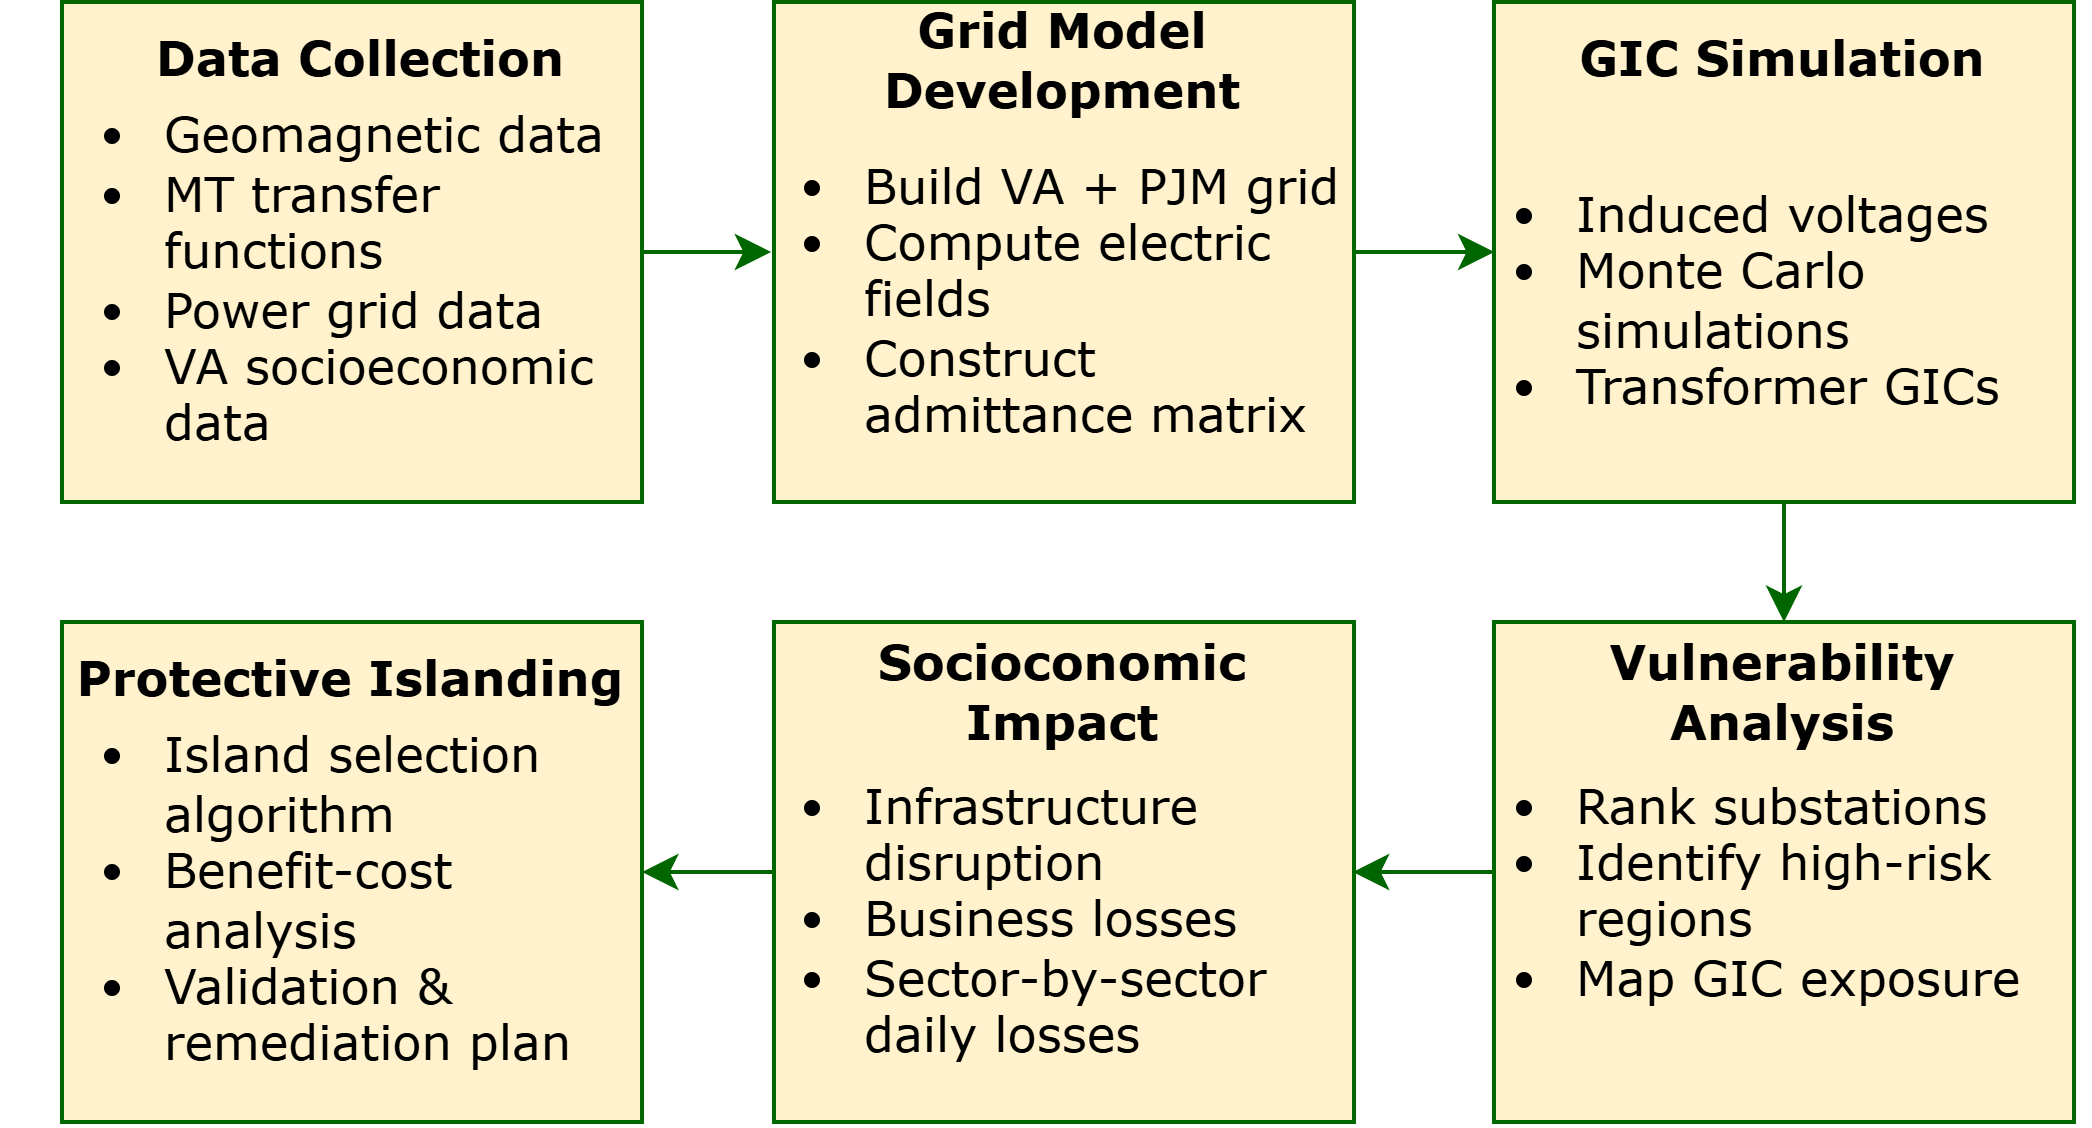
\includegraphics[width=0.8\textwidth]{Figures/VAMethodology.png}
  \caption{Flowchart of methodology for VA adaptation of C-SWIM and data-driven mitigation}
  \label{fig:methodology}
\end{figure}

\subsection{Study Domain and Network Construction}

While impact assessment was focused on the state of Virginia, the constructed electrical model needs to extend past state borders. GICs move through interconnected transmission lines across state borders, meaning that the current flowing through Virginia substations is dependent on the network topology of surrounding states. As such, the present work's study domain was defined as the entire PJM footprint, PJM being a regional transmission organization (RTO) that encompasses thirteen states, including Virginia, and the District of Columbia. Building the network outside of the PJM interconnection was determined to be unnecessary, since electrical connections between RTOs are weak and since PJM boundaries are at a distance from Virginia such that extension would contribute little change to the simulation. All grid vulnerability results, though evaluated for PJM, are filtered for Virginia.

The Virginia-PJM power grid was constructed via open-source data, following \citeA{oughton2026reproduciblemethodmappingelectricity}, as opposed to splicing from the national power grid. This ensures that the electrical model is constructed with a documentable, transferable process, supporting the goal of a reproducible framework for analysis of any power grid region. Extra-high-voltage (EHV) transmission lines were defined to be $\geqslant 230 kV$ and were derived from Homeland Infrastructure Foundation-Level Data (HIFLD), spatially filtered to the PJM region. EHV substation locations were determined through OpenStreetMap (OSM) via an Overpass API, and transmission line endpoints were snapped to the nearest substations within a fixed threshold distance. The result was a topologically connected network and disjointed components that were logged. Each substation was assigned a unique identifier, while transmission lines were assigned a length computed from geometry and resistance determined by voltage level.

The resulting network comprises of 2,728 substations and 4,587 transmission lines (Figure~\ref{fig:VAnetwork}). This replaces the national grid model as the input to every downstream stage in the adapted pipeline.



\begin{figure}[h]
  \centering
  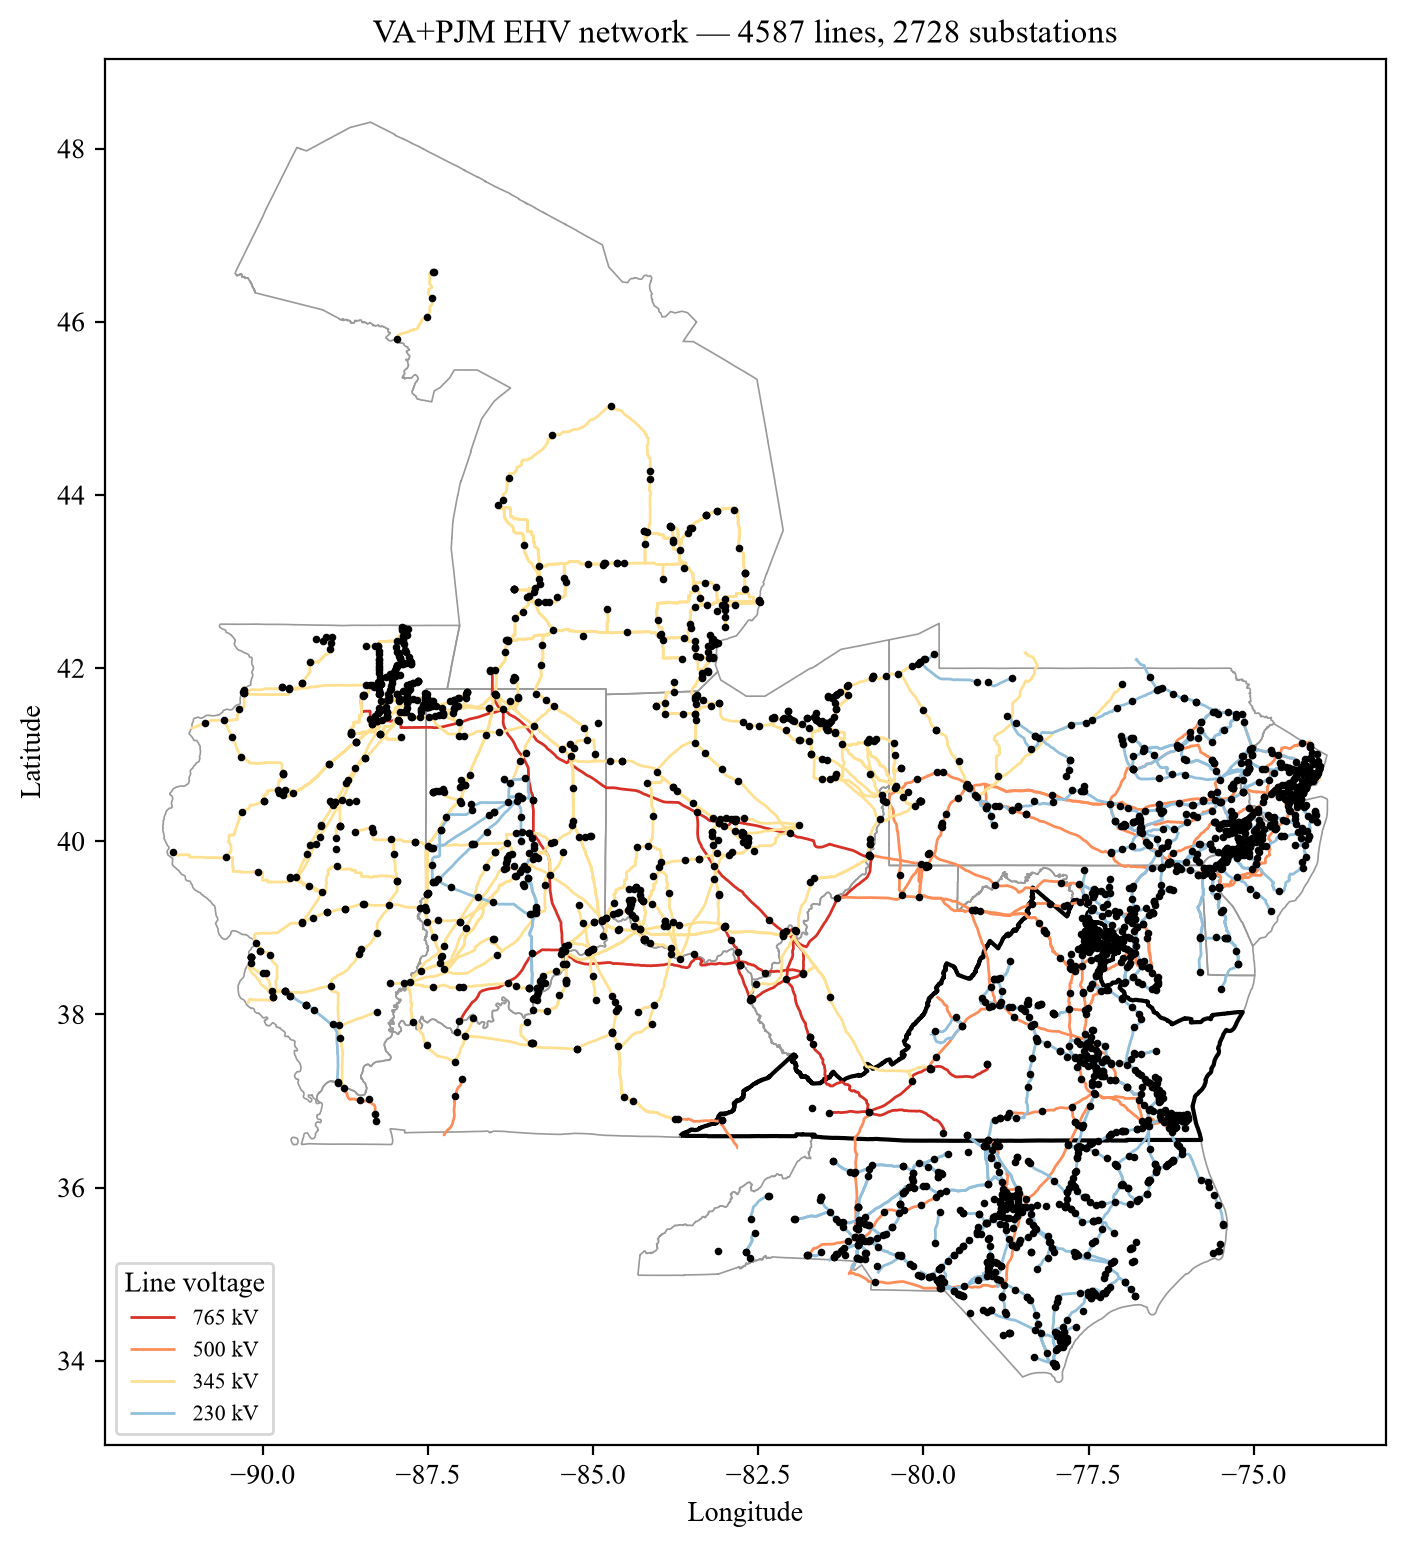
\includegraphics[width=0.7\textwidth]{Figures/va_pjm_network.png}
  \caption{Virginia + PJM power grid constructed with OSM and HIFLD data}
  \label{fig:VAnetwork}
\end{figure}

\subsection{Geoelectric Hazard Characterization}

The geoelectric field induced at Earth's surface by geomagnetic storms is characterized by the 92 historical storms used in the national C-SWIM pipeline. Derivation of the geoelectric field follows the two-stage approach in Section~\ref{sec:litreview}: SECS interpolation uses ground-magnetometer data to determine the geomagnetic field \citeA{Rigler2019}, and convolution with magnetotelluric transfer functions yields the geoelectric field, following \citeA{Lucas2020}. Critically, this chain is only dependent on the geomagnetic observatory network, not the underlying grid topology, so it was inherited directly from the national pipeline without modification.

Because of this topology independence, the interpolation was run across all 1,696 magnetotelluric sites rather than being restricted to Virginia. Regional filtering would not only be unnecessary, but also a deviation from the validated method. Including sites well beyond the study domain also ensures sufficient anchoring for accurate interpolation.

Storm scenarios in this work were constructed and classified by return period. For every transmission line and site in the study domain, peak geoelectric amplitudes are determined for each of the 92 historical storms, a lognormal distribution being fit to these maxima. The fit is then extrapolated to recurrence intervals spanning from 50- to 250-year geomagnetic storm scenarios. These are synthetic storm scenarios, meaning they are statistically pooled and not specific to any single historical storm. For real-world validation beyond these synthetic storms, named historical storms are used: the May 2024 Gannon storm, the Halloween Storm, and St.~Patrick's Day Storm.

It is important to note that the specific historical storms have real use in this work for evaluating mitigation through protective islanding. While synthetic scenarios inherit the per-line field magnitude from an independent statistical fit, they inherit per-line orientation only from the Gannon storm. This means that all return-period scenarios have the same directional signature, and the specific historical storms are needed to evaluate how different directional signatures impact mitigation. 

\subsection{Line-Voltage Recomputation}

A critical distinction governs which facets of the national pipeline can be directly replicated and which must be modified. As established earlier, interpolated geomagnetic and geoelectric field values are topology-independent and can therefore be measured in the same manner as the national pipeline without recomputation.

Line-level induced voltages, however, are critically dependent on grid topology. Following \citeA{BotelerGIC}, the voltage induced along a transmission line is the integral of the geoelectric field along that line's specific path, depending on a line's length, orientation, and endpoints. Since these voltages are bound to specific line identifiers, they are inseparable from the underlying network topology. As such, the induced voltages for the Virginia-PJM power grid have no analog in the national output to subset.

Consequently, line-voltage was recomputed for the Virginia-PJM line set, integrating the (reused) geoelectric field along each of the newly constructed lines across all storm scenarios. This constitutes a general finding regarding regional adaptations of national GIC pipelines: while field computation can be directly transferred, line-level products are topology-specific and must be recomputed. Making this distinction is critical in a regional adaptation to avoid unnecessary recomputation and invalid reuse. 

\subsection{GIC Solve}

After building the network topology and computing induced line voltages, GICs were computed by solving the network as a resistive DC circuit. The nodal admittance (Y) matrix was built to represent power grid topology of the Virginia-PJM region using real line resistances and substation grounding parameters, following the modified Lehtinen-Pirjola (LPm) formulation presented in \citeA{LPm2022}. Given induced line voltages as driving sources, the solve yields nodal voltages, branch currents, and neutral-to-ground currents.

Performing a single GIC solve faces a methodological barrier: exact transfomer configurations are not publicly available at the substation level. Following the national pipeline, a Monte Carlo procedure was used for 3,000 iterations of sampled transformer configurations (autotransformer, wye-wye, and wye-delta), the number of transformer units per substation, and grounding resistances. Running the GIC solve for each Monte Carlo iteration yielded a distribution of GIC values at each substation rather than a single estimate, the point estimate and 95th-percentile values being used for vulnerability analysis. 

To measure GIC, both winding and neutral-to-ground currents are computed. The effective per-phase winding GIC is adopted as the risk-ranking quantity, as it more directly represents the thermal stress experienced by transformer windings than neutral-to-ground current alone \cite{Klauber2020AGE}.

\subsection{Vulnerability \& Economic Analysis}

The GIC distributions are translated into transformer failure probabilities using continuous fragility curves. Following the approach in Section~\ref{sec:litreview}, failure probability is modeled as a lognormal function of effective per-phase winding GIC, anchored to the NERC TPL-007 benchmark of 75~A/phase above which transformers require thermal assessment \cite{NERC2014}. Specifically, the failure probability of a transformer experiencing an
effective per-phase GIC of $I_E$ is
\begin{equation}
P_f(I_E) = \Phi\!\left(\frac{\ln I_E - \mu}{\sigma}\right),
\label{eq:fragility}
\end{equation}
where $\Phi$ is the standard normal cumulative distribution function and
$\mu$ and $\sigma$ are the fragility parameters anchored to the 75~A/phase
benchmark. A continuous fragility curve is much more suitable for this work than binary thresholding, enabling every increment of GIC to contribute to failure probability. This becomes critical when evaluating protective islanding, in which small magnitudes of GIC redistribution can notably impact transformer failure likelihood. 


In order to translate substation failure into economic and human impact, a spatial link between grid regions and their surrounding economic activity must be created. Following \citeA{Thacker2017}, Voronoi tesselation was used to construct service territories around each substation, divided based on proximity. Population and economic output, derived from ZIP Code Tabulation Area (ZCTA) census and economic data, were then allocated within these territories by dasymetric interpolation against National Land Cover Database (NLCD) land cover, apportioning activity to inhabited land as opposed to assuming uniformity. This approach enables a specific substation's failure to be linked to the population and establishments it serves. 

In order to assess economy-wide impact, localized losses are translated into sectoral propagation through input-output (IO) modeling. Three formulations were applied: a supply-side Ghosh value-added model, a demand-side Leontief consumption model, and a combined Leontief consumption-plus-production model, which is used for this work's primary results. Each approach models economic propagation differently, and taken together, the range of plausible impact can be bounded. 

The methodology for economic analysis does have a scope limitation. The IO analysis in this work uses a national social accounting matrix (SAM) and technology tables driven by Virginia-specific supply and demand shock. Construction a Virginia-specific SAM was out of the scope of this work, and this exclusion is consistent with common practice in sub-national disaster economics, where regional shocks are applied to national inter-industry structure.

\subsection{Protective Islanding}

An algorithmic approach to protective islanding was implemented in this work for GIC mitigation. Protective islanding intentionally isolates a portion of the network, leaving it without power for a short duration to prevent substation failure. The network is reconnected after this short period, potentially avoiding the long lead times of transformer replacement. 

This work evaluated three original algorithms for island selection, yielding three unique islands that were run through cost-benefit analysis. 

\subsubsection{Island A: Betweenness Centrality}\label{sec:methodA}

The selection algorithm for Island A, the first tested island, is outlined in Figure~\ref{fig:method1}, with symbols defined in Table~\ref{tab:islanding-legends}. The algorithm is characterized by its use of betweenness centrality from Section~\ref{sec:litreview} in the formulation of the Substation Criticality Index (SCI), an indicator of a substation's relative importance. The algorithm follows a greedy, seeded approach, where island formation begins at the substation with the greatest SCI and repeatedly appends a neighboring substation until no neighboring substation increases the ratio between the island's aggregate SCI and switching cost. 

\subsubsection{Island B: Current-flow Betweenness Centrality \& Redistribution Measurement}\label{sec:methodB}

The selection algorithm for Island B addressed two deficits in the selection algorithm for Island A. First, current-flow betweenness was used instead of betweenness centrality as a better proxy for how current flows through a graph. Second, a measure of redistribution was introduced since intervention at one portion of a network can impact the surrounding network, as established in Section~\ref{sec:litreview}. The algorithm is outlined in Figure~\ref{fig:method2}, while symbols are defined in Table~\ref{tab:islanding-legends}.


\subsubsection{Island C: Current-flow Betweenness \& Historical Storm Admittance Solve}\label{sec:methodC}
The selection algorithm for Island C addresses a key deficit of the selection algorithms of Island A and Island B: real storms have directionality, while GIC distribution proxies such as betweenness centrality or current-flow betweenness do not respect specific directions. Island C incorporates admittance matrix solves for three historical storms to narrow the substation pool and evaluate islands. The algorithm is outlined in Figure~\ref{fig:method3} while symbols are defined in Table~\ref{tab:islanding-legends}.

\subsubsection{Economic Evaluation Methodology}

Economic evaluation for each island focused on measuring the economic difference between the fragility outputs of the islanded and non-islanded topologies. Both the baseline and islanded topologies were solved for GIC and run through the pipeline's fragility assessment, which in turn led to two separate economic assessments. This was repeated across synthetic return periods and historical storms and yielded a difference in terms of GDP loss per day, enabling cost-benefit analysis.

Key assumptions were made for the economic evaluation. Firstly, a 6-hour disconnection period was assumed, consistent with the typical several-hour main-phase duration of a geomagnetic storm \cite{gonzalez1994geomagnetic}, meaning that the islanded topology was only active for 6 hours before reverting to the original topology. This allowed islanding to potentially lower the risk of transformer failure without causing long-term disconnection that would incur severe economic losses. The economic loss of the 6 hours for the disconnected portion was accounted for in island evaluation.

To translate daily economic losses into a single economic benefit estimate, damaged transformer replacement times needed to be considered. Reported large power transformer procurement lead times of roughly one to two years \cite{doe2014lpt} informed an economic analysis built with three potential replacement times: 180 days, representing fast response; 365 days, representing a moderately quick response; and 730 days, representing a slow response. The results in this work are reported for a 365-day replacement time, but it should be noted that this assumption affects the magnitude but not the existence of benefit.

To estimate cost, a \$0.025M switching cost was assumed per line, an order of magnitude consistent with switching-cost estimates from a comparable islanding mitigation study of New Zealand's power network \cite{oughton2026assessingeconomicbenefitsspace}, and this cost was counted for switching into an islanded formation as well as switching out of it.

The economic benefit was the GDP difference, as determined by the Ghosh input-output model, between the fragility outputs of the islanded and non-islanded topologies over the transformer replacement period. The cost included loss-of-power for the islanded region and switching cost. The benefit-cost ratios were calculated as the quotient of economic benefit and cost.



\begingroup
\footnotesize
\begin{longtable}{c c p{9.5cm}}
\caption{Symbol definitions for the three islanding selection methods: A (betweenness-centrality SCI, Section~\ref{sec:methodA}), B (current-flow betweenness with redistribution measurement, Section~\ref{sec:methodB}), and C (current-flow-betweenness discovery with real-storm admittance scoring, Section~\ref{sec:methodC}).}
\label{tab:islanding-legends}\\
\toprule
\textbf{Method} & \textbf{Symbol} & \textbf{Definition} \\
\midrule
\endfirsthead
\multicolumn{3}{l}{\textit{Table~\ref{tab:islanding-legends} continued}} \\
\toprule
\textbf{Method} & \textbf{Symbol} & \textbf{Definition} \\
\midrule
\endhead
\midrule
\multicolumn{3}{r}{\textit{continued on next page}} \\
\endfoot
\bottomrule
\endlastfoot
\multirow{9}{*}{A} & $G$ & Power grid network graph (substations as nodes, transmission lines as edges) \\
 & $b_i$ & Betweenness centrality of substation $i$ \\
 & $r_i$ & Normalized geomagnetically-induced-current (GIC) risk of substation $i$ \\
 & $e_i$ & Normalized economic exposure of substation $i$ (population and GDP density) \\
 & $\text{SCI}_i$ & Composite substation criticality index --- weighted combination of $b_i$, $r_i$, $e_i$ \\
 & $S$ & Set of eligible substations (grid-connected, within the study region) \\
 & $V$ & Total criticality value of the candidate island, $V = \sum_{i \in \text{island}} \text{SCI}_i$ \\
 & $C$ & Switching cost of the candidate island's boundary lines \\
 & $R$ & Benefit-cost ratio, $R = V / C$ \\
\midrule
\multirow{10}{*}{B} & $G$ & Power grid network graph (substations as nodes, transmission lines as edges) \\
 & $r_i$ & Normalized geomagnetically-induced-current (GIC) risk of substation $i$ \\
 & $e_i$ & Normalized economic exposure of substation $i$ (population and GDP density) \\
 & $w_i$ & Risk weight of substation $i$, $w_i = 0.5\,r_i + 0.5\,e_i$ \\
 & $\text{cfb}_i$ & Current-flow betweenness centrality of substation $i$, recomputed before and after a candidate cut \\
 & $\text{benefit}$ & Sum of $w_i$ over the candidate island's own members \\
 & $\text{redistribution\_cost}$ & Weighted increase in current-flow betweenness at substations outside the island, caused by the cut \\
 & $\text{switching\_cost}$ & Cost of switching the candidate island's boundary lines \\
 & $\lambda,\ \mu$ & Weighting coefficients balancing redistribution cost and switching cost against benefit \\
 & $\text{net\_score}$ & $\text{benefit} - \lambda \cdot \text{redistribution\_cost} - \mu \cdot \text{switching\_cost}$ \\
\midrule
\multirow{9}{*}{C} & $G$ & Power grid network graph (substations as nodes, transmission lines as edges) \\
 & $w_i$ & Risk weight of substation $i$ (GIC risk and economic exposure), used only to help discover candidates \\
 & $\text{cfb}_i$ & Current-flow betweenness centrality of substation $i$, used only to widen candidate discovery, never to score a candidate \\
 & $\text{own\_effect}$ & Fragility-weighted change in expected GDP loss at the candidate island's own members, for one real historical storm \\
 & $\text{redistribution\_cost}$ & Fragility-weighted change in expected GDP loss at substations outside the island, for one real historical storm \\
 & $\text{worst\_case}$ & The largest (most unfavorable) $\text{own\_effect} + \text{redistribution\_cost}$ across the three real historical storms considered \\
 & $\varepsilon$ & Required safety margin: a candidate is only accepted if $\text{worst\_case} \le -\varepsilon$ \\
 & $\mu$ & Weighting coefficient applied to switching cost \\
 & $\text{net\_score}$ & $-\text{worst\_case} - \mu \cdot \text{switching\_cost}$, computed only for candidates that already pass the hard filter \\
\end{longtable}
\endgroup

\begin{figure}[!ht]
  \noindent\makebox[\textwidth][c]{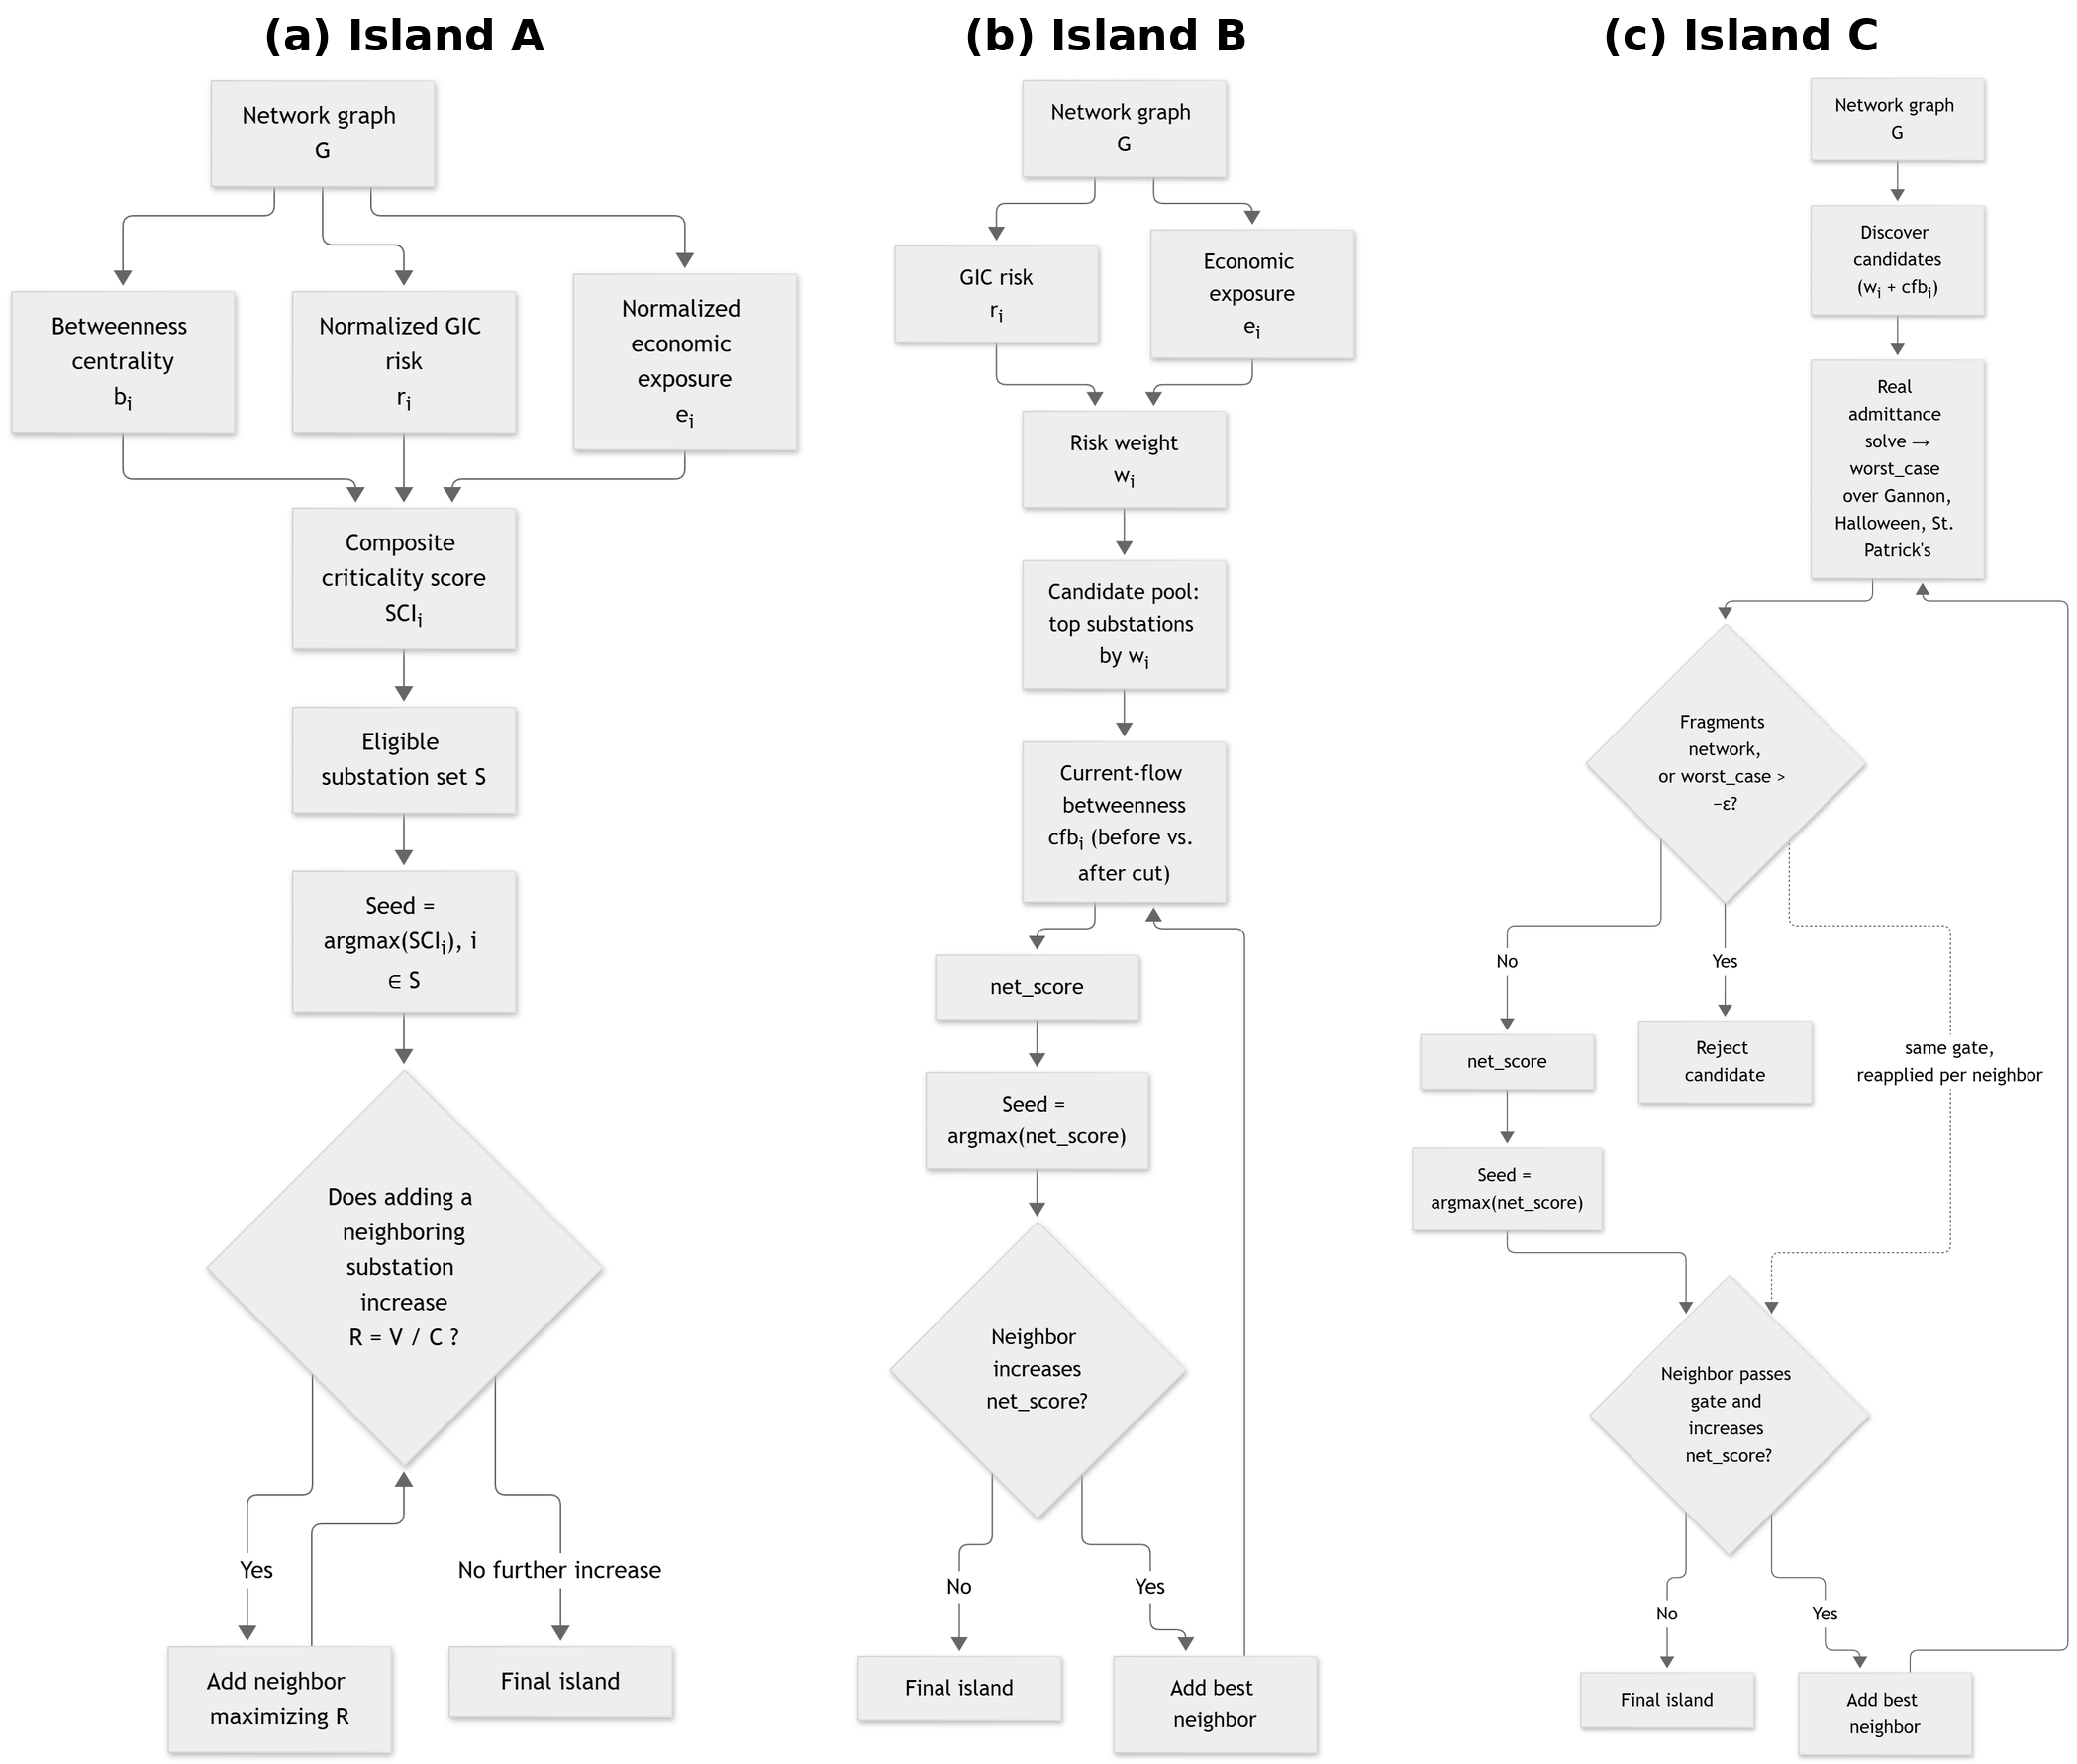
\includegraphics[width=7.0in]{Figures/va_island_methods_combined.png}}
  \caption{Flowcharts for island selection algorithms}
  \label{fig:method3}
\end{figure}


\addcontentsline{toc}{section}{Acknowledgments}
\clearpage
\section{Results}

\begin{figure}[!ht]
  \centering
  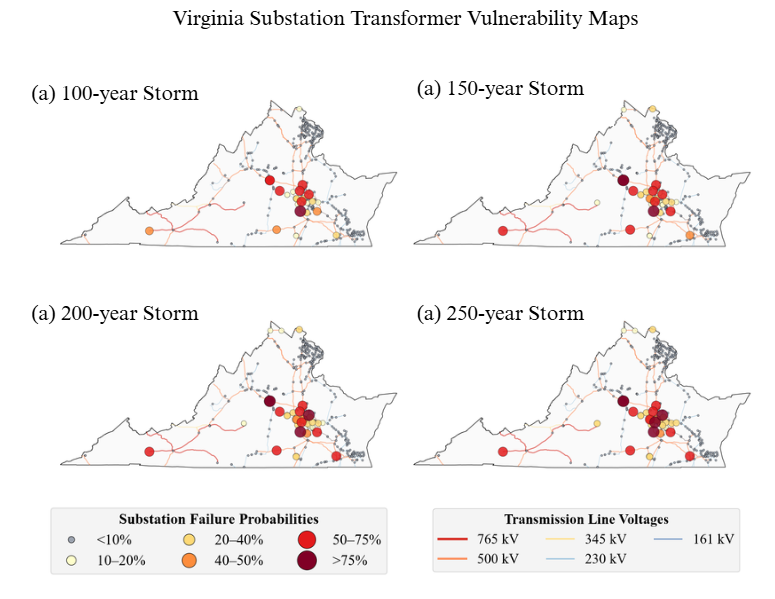
\includegraphics[width=0.8\textwidth]{Figures/trafosmap.png}
  \caption{Spatial map of transformer failure probability for varying storm scenarios.}
  \label{fig:transformerfailure}
\end{figure}

\begin{figure}[!ht]
  \centering
  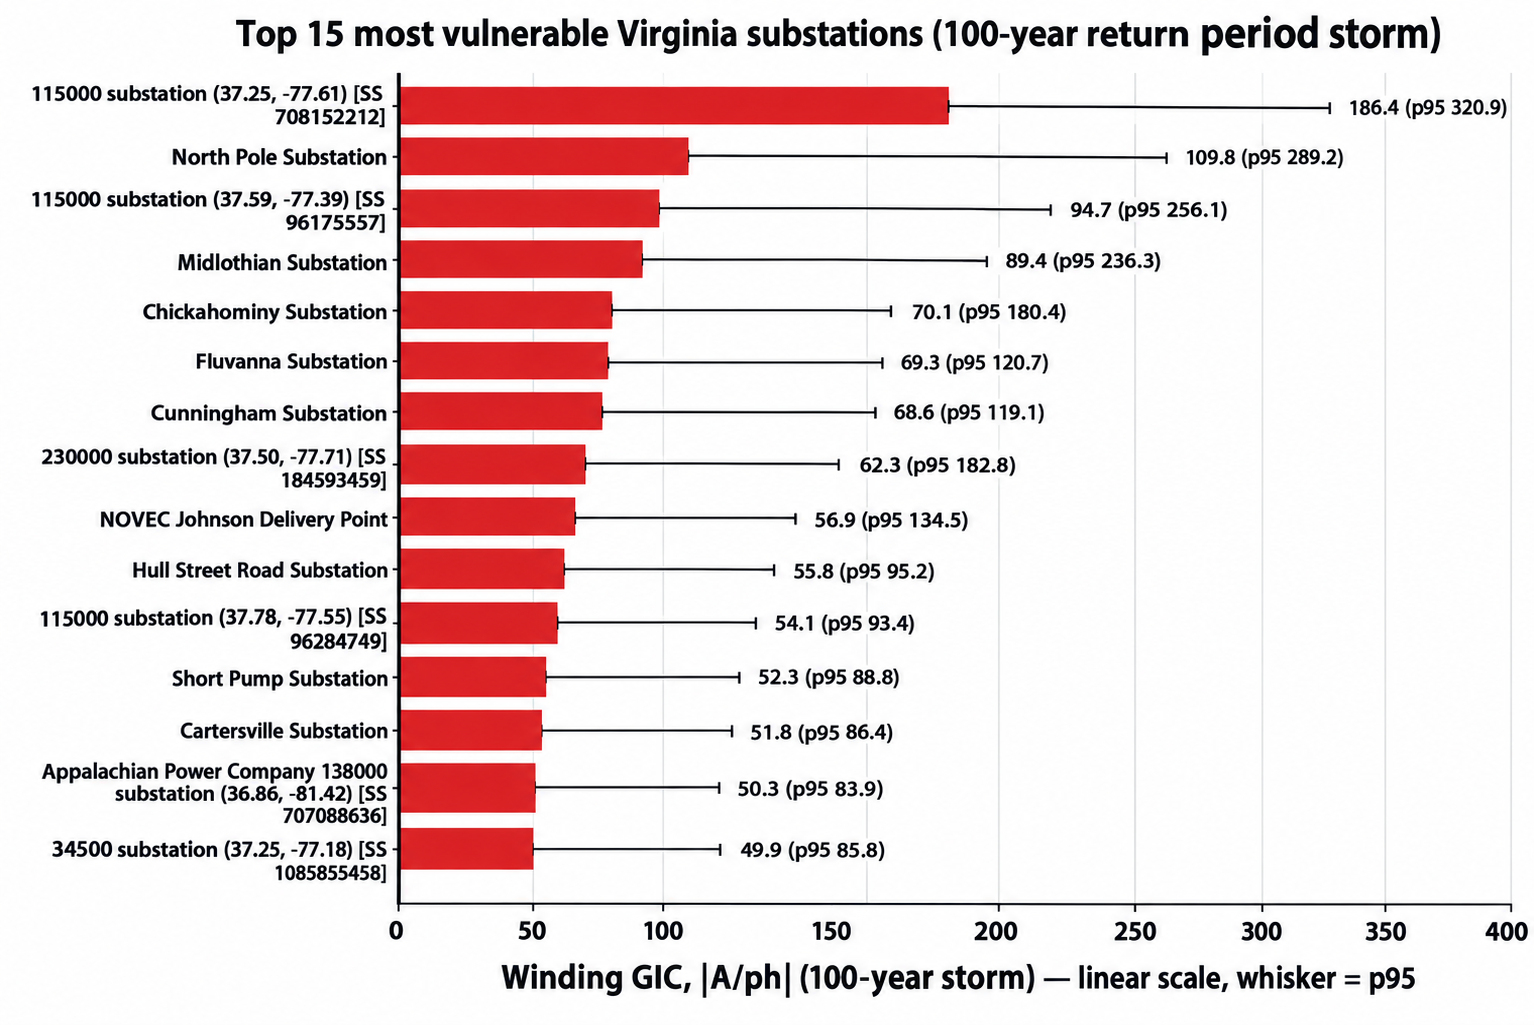
\includegraphics[width=0.9\textwidth]{Figures/top15va.png}
  \caption{Top at-risk substations based on winding GIC.}
  \label{fig:subsranking}
\end{figure}


\begin{figure}[h]
  \centering
  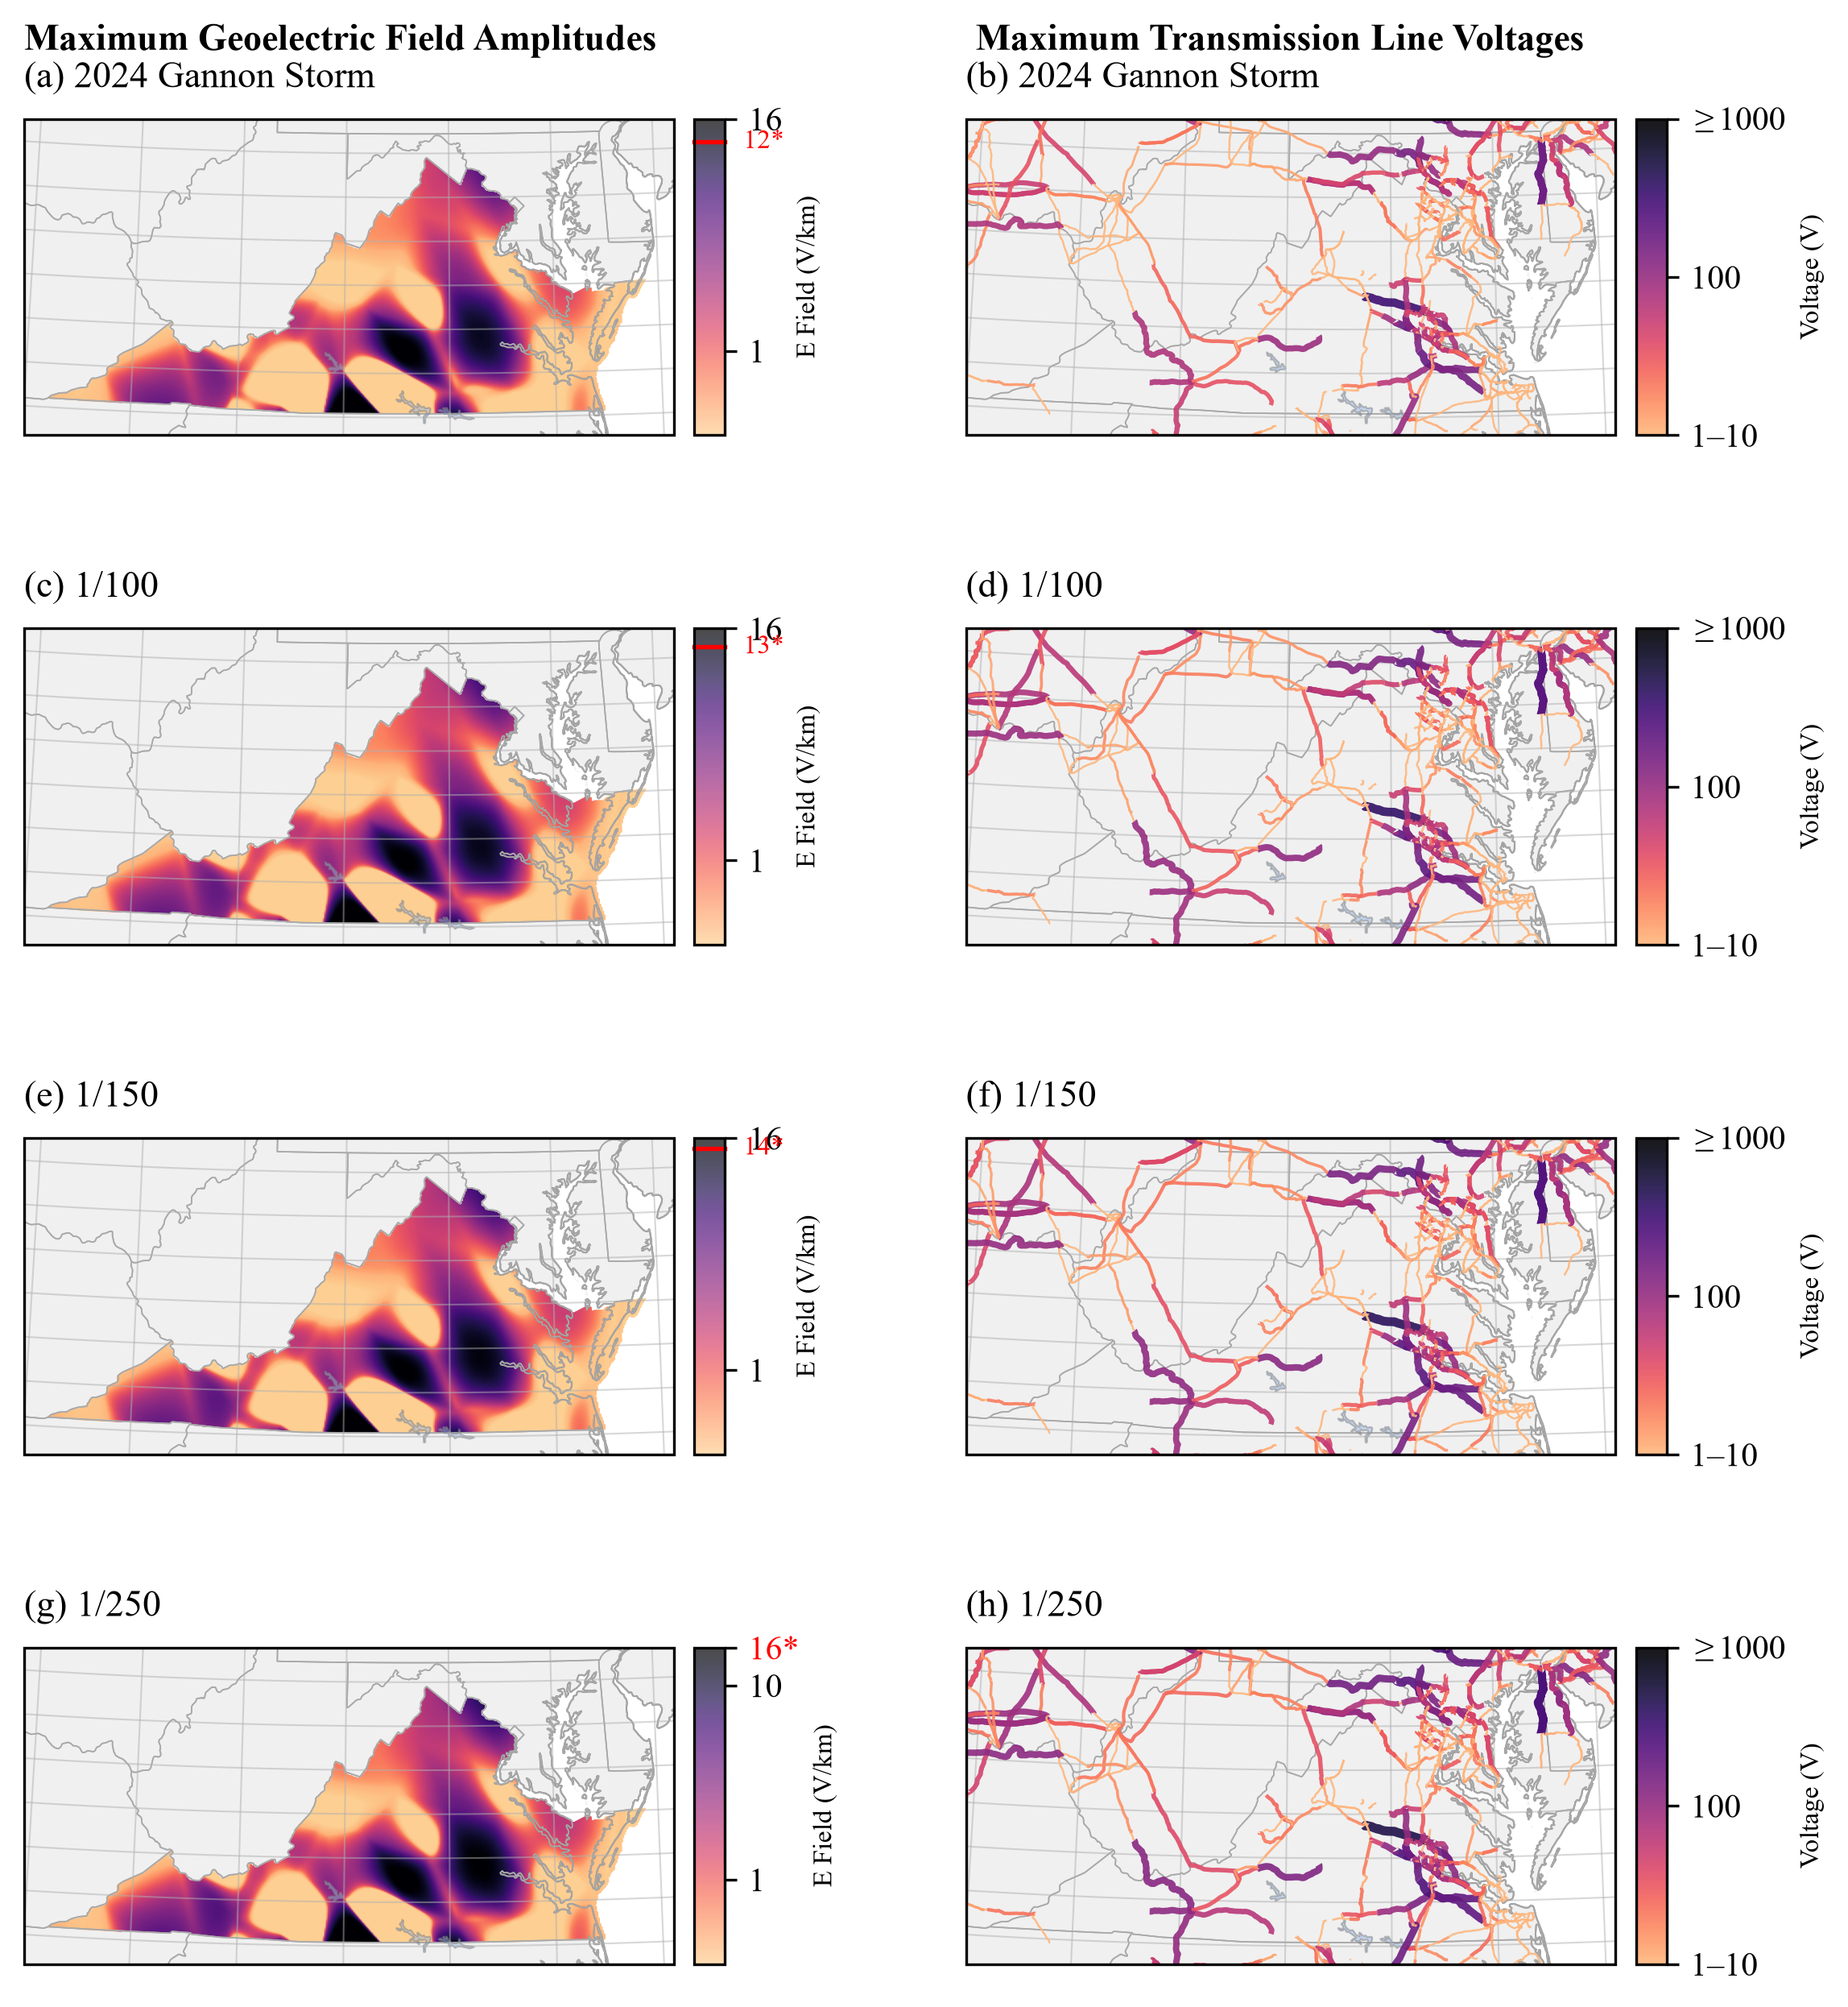
\includegraphics[width=\textwidth]{Figures/va_hazard_maps.png}
  \caption{E-field and induced transmission line voltages for varying storm scenarios}
  \label{fig:hazardmap}
\end{figure}
Since the pipeline resolves geomagnetically induced currents down to the transformer, risk can be assessed for individual substations, the level of precision at which mitigation occurs. Figure~\ref{fig:transformerfailure} shows a spatial map of transformer failure likelihood for different return periods constructed using lognormal fragility curves with respect to effective per-phase GIC. The results reveal that estimated risk is heavily concentrated in central Virginia, particularly in the Richmond region (37.54083° N, -77.43667° W). This is consistent with a relatively large estimated geolectric field amplitude for the region (Figure~\ref{fig:hazardmap}) and the intersection of many high-voltage corridors in the Richmond area (Figure~\ref{fig:VAnetwork}). 

A ranking of Virginia substations based on absolute winding GIC is shown in Figure~\ref{fig:subsranking}. The substation at (37.25°N, 77.61°W) had a significantly higher winding GIC than the other substations, and many of the most at-risk substations are located near the Richmond area. This ranking is the single most operationally actionable output of the assessment: it identifies, by name and location, the specific substations a transmission operator or state energy office would prioritize for monitoring, hardening, or targeted mitigation
\begin{figure}[h]
  \centering
  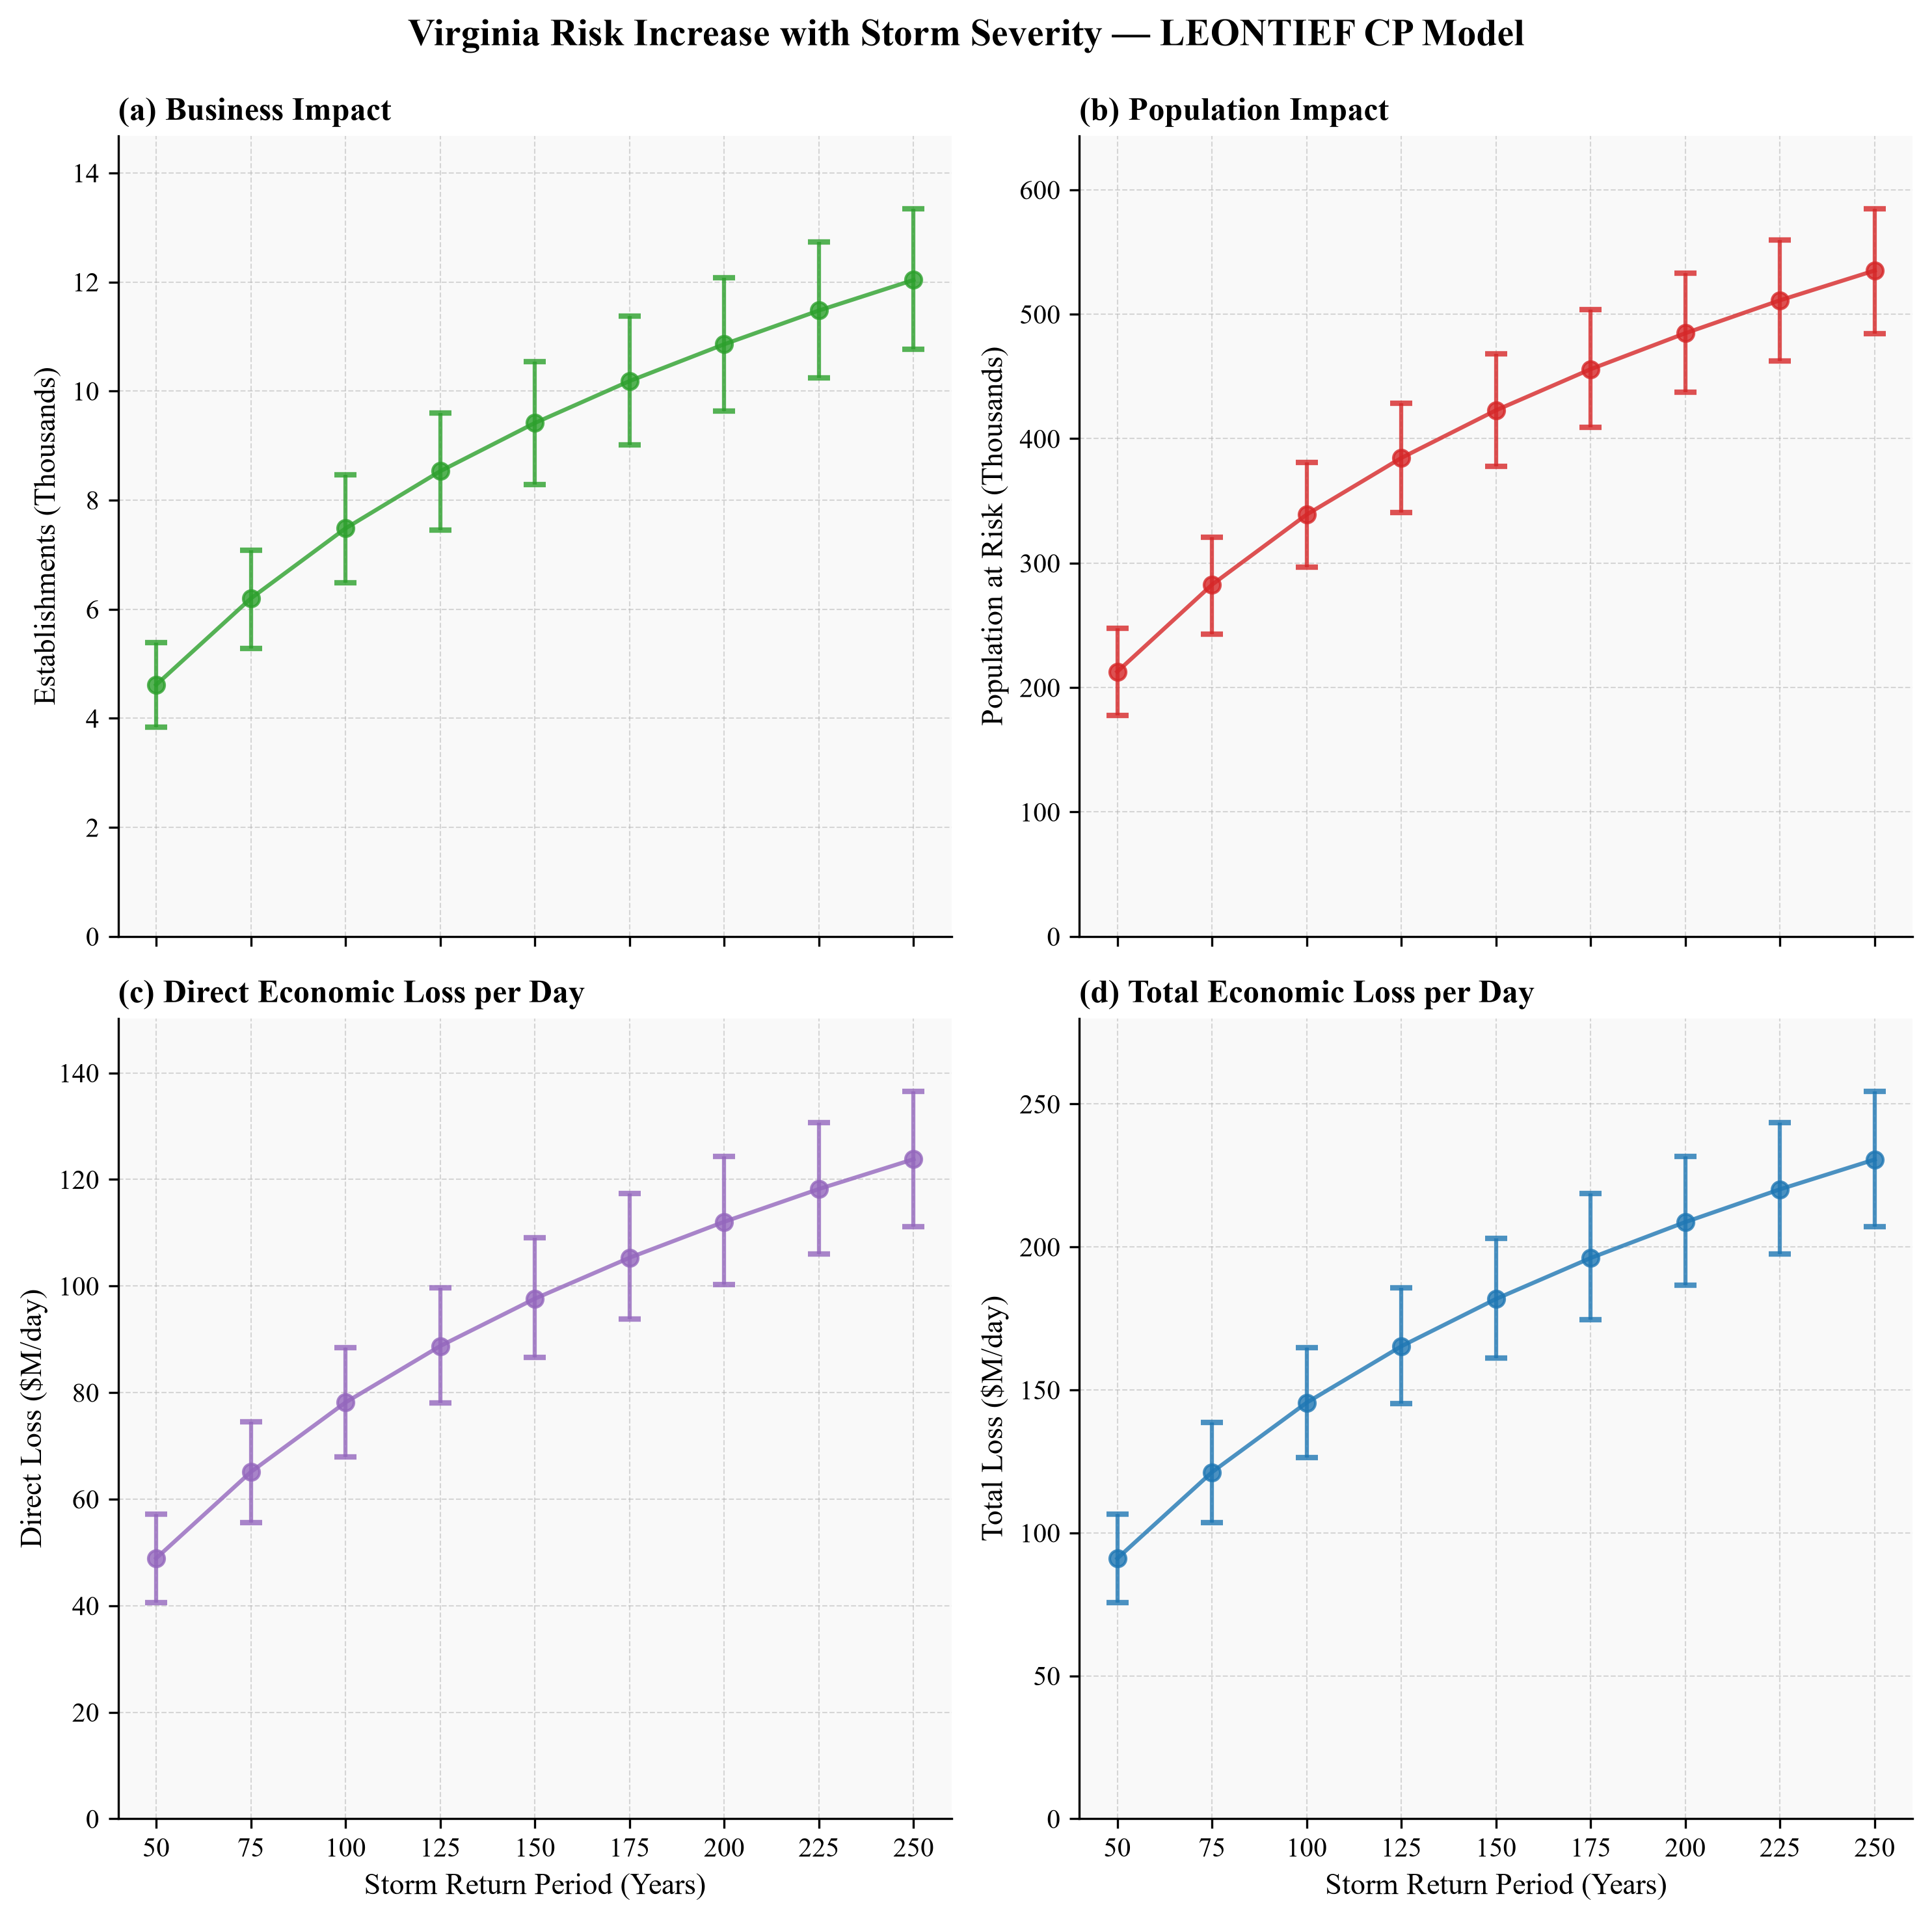
\includegraphics[width=\textwidth]{Figures/va_severity_risk_leontief_cp.png}
  \caption{Severity risk for varying return periods via Leontief Consumption + Production IO modeling}
  \label{fig:severityrisk}
\end{figure}
\begin{table}[h]
\centering
\caption{Estimated daily economic and human impact on Virginia by storm
return period, and for the 2024 Gannon storm (Leontief consumption +
production model). Losses are reported as mean $\pm$ standard deviation in
millions of dollars per day; population and establishments at risk are in
thousands.}
\label{tab:econ_impact}
\resizebox{\textwidth}{!}{%
\begin{tabular}{lcccc}
\hline
Return period & Total loss (\$M/day) & Direct loss (\$M/day) & Pop.\ at risk (k) & Establishments at risk (k) \\
\hline
100-year      & $145.5 \pm 19.1$ & $78.1 \pm 10.2$ & 339 & 7.5 \\
150-year      & $181.8 \pm 21.0$ & $97.6 \pm 11.3$ & 423 & 9.4 \\
200-year      & $208.7 \pm 22.3$ & $112.0 \pm 11.9$ & 485 & 10.9 \\
250-year      & $230.6 \pm 23.7$ & $123.8 \pm 12.6$ & 535 & 12.0 \\
Gannon (2024) & $137.8 \pm 9.8$  & $73.8 \pm 5.2$   & 323 & 6.4 \\
\hline
\end{tabular}%
}
\end{table}



\begin{figure}[!ht]
  \centering
  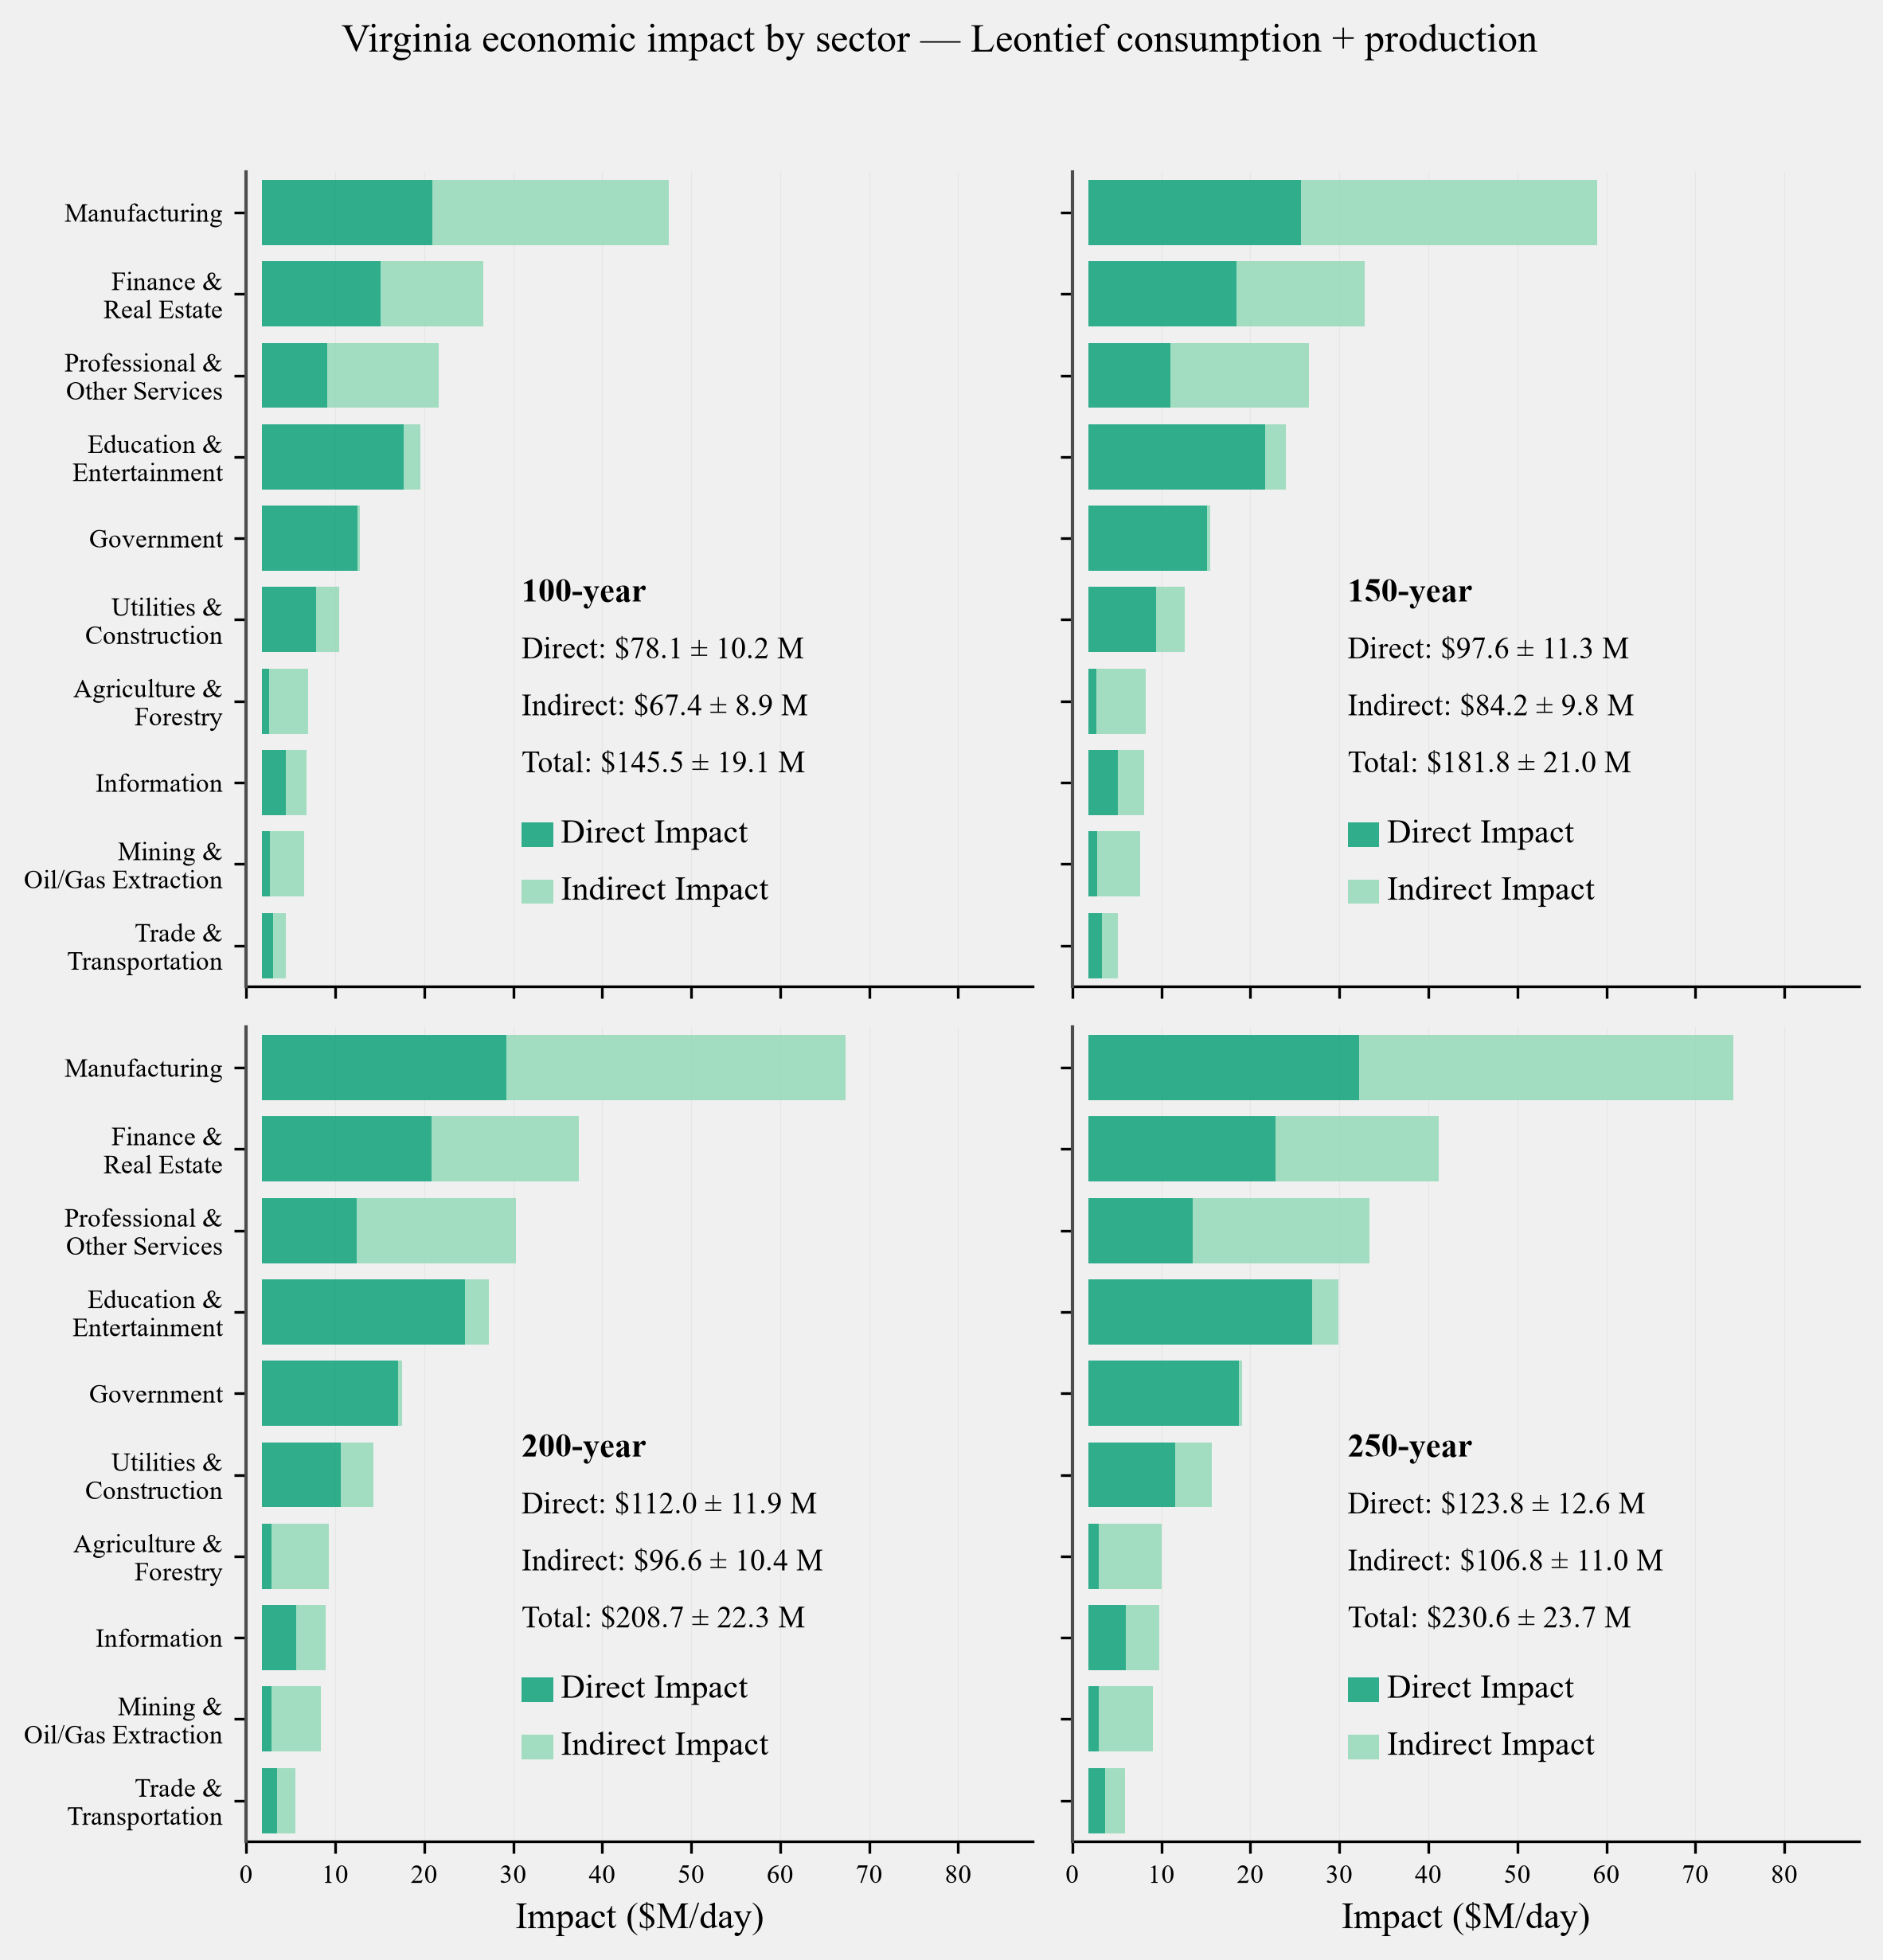
\includegraphics[width=\textwidth]{Figures/va_econ_impact_leontief_cp.png}
  \caption{Sector-by-sector daily loss estimates from Leontief consumption + production under varying storm scenarios}
  \label{fig:LeontiefCP}
\end{figure}

Beyond physical vulnerability, the pipeline quantifies socioeconomic impact through input-output modeling. Figure~\ref{fig:severityrisk} and Table~\ref{tab:econ_impact} report daily economic losses and human impact under the Leontief consumption + production model for varying return periods. For a 100-year storm, the estimated daily economic loss is \$145.5M, while loss grows to \$230.6M under a 250-year storm, with 535,000 individuals and 12,000 establishments at risk. General risk increases systematically with return period, though the rate of change diminishes over return period, suggesting a plateauing effect beyond which increasing return period does little to increase risk. Notably, the May 2024 Gannon Storm yielded an estimated daily loss of \$137.8M, just under the severity of a 100-year storm, grounding the return-period estimates in a real storm. Critically, indirect (inter-industry) losses accounted for an average of ~46\% of total daily losses across tested return periods.

The sectoral decomposition presented in Figure~\ref{fig:LeontiefCP} reveals that manufacturing and finance \& real estate are the most affected sectors, consistent with findings from the national pipeline. Manufacturing alone accounts for the largest share, driven predominantly by indirect supply-chain effects.

The economic results also show that Virginia is particularly at risk to geomagnetic storms. Despite comprising ~2.5\% of national gross domestic product, the pipeline estimates daily losses for Virginia under a 250-year storm to be ~11\% of the national pipeline's point estimate of \$2.04B under the same scenario. This means that Virginia is estimated to be at over a four-times risk factor relative to uniform distribution by state. 

\begin{figure}[!ht]
  \centering
  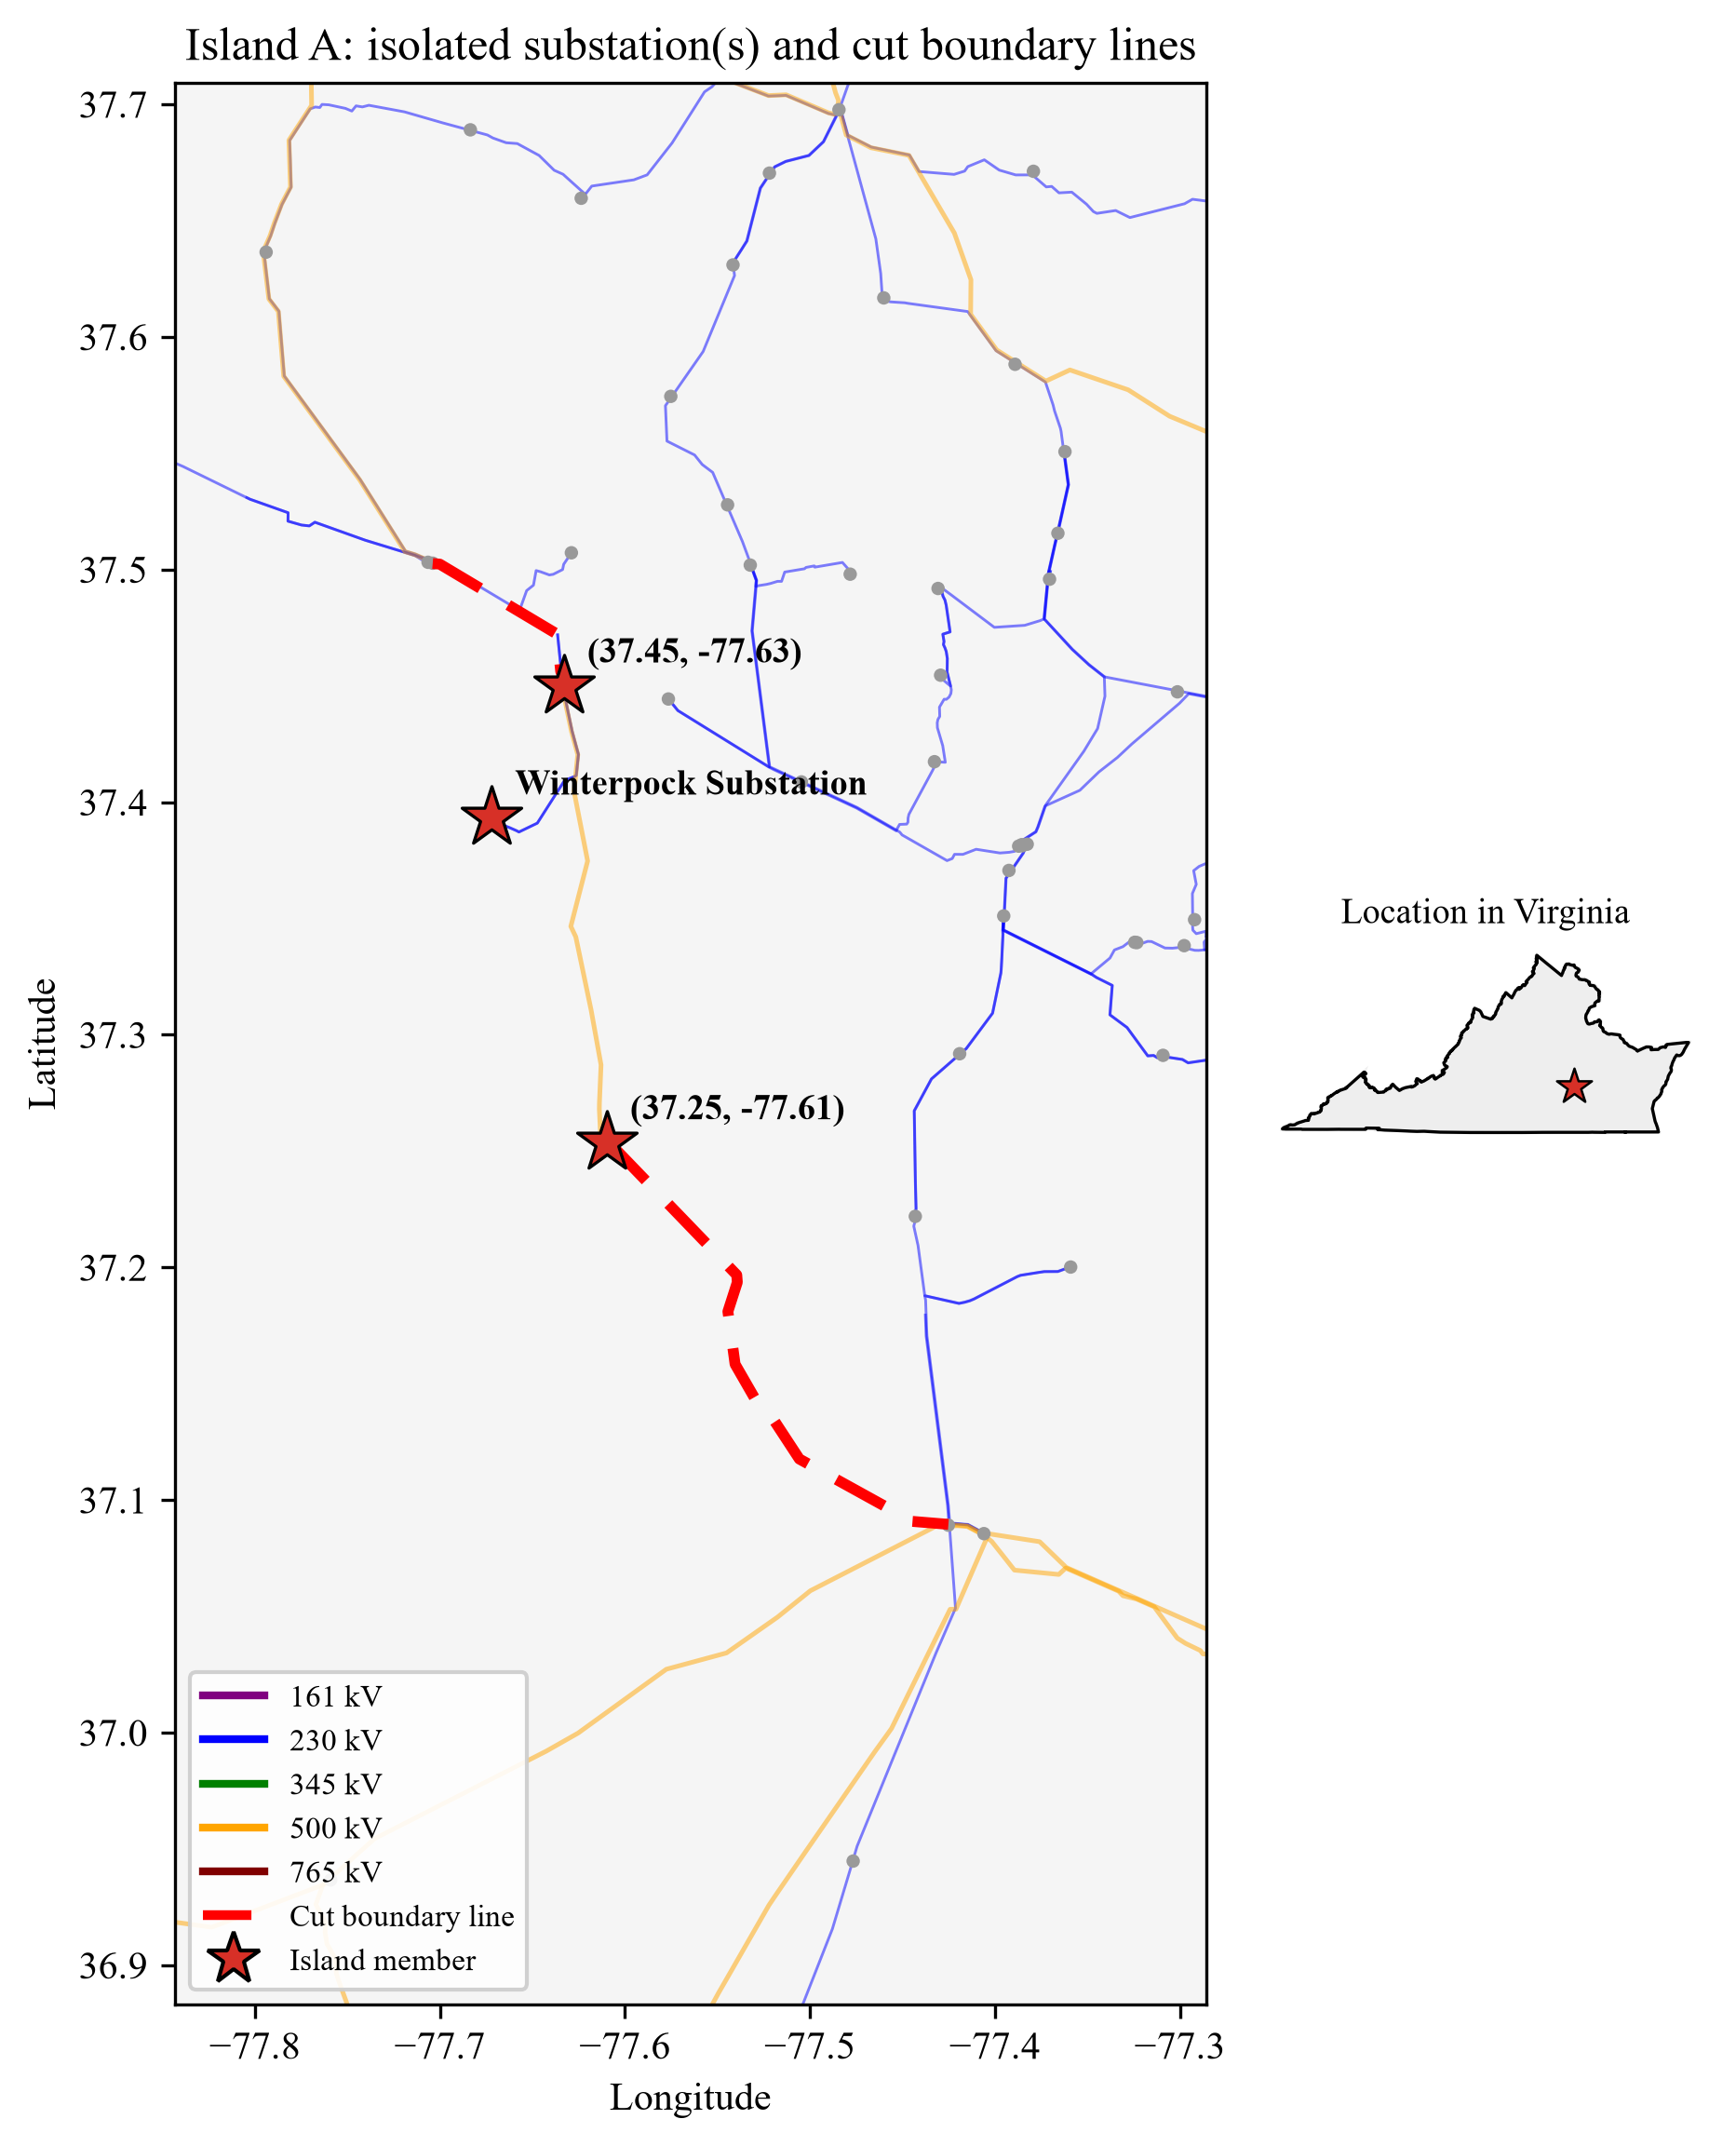
\includegraphics[width=\textwidth]{Figures/va_island_a_map.png}
  \caption{Map of Island A substations and boundary cuts.}
  \label{fig:islandA}
\end{figure}
\begin{figure}[!ht]
  \centering
  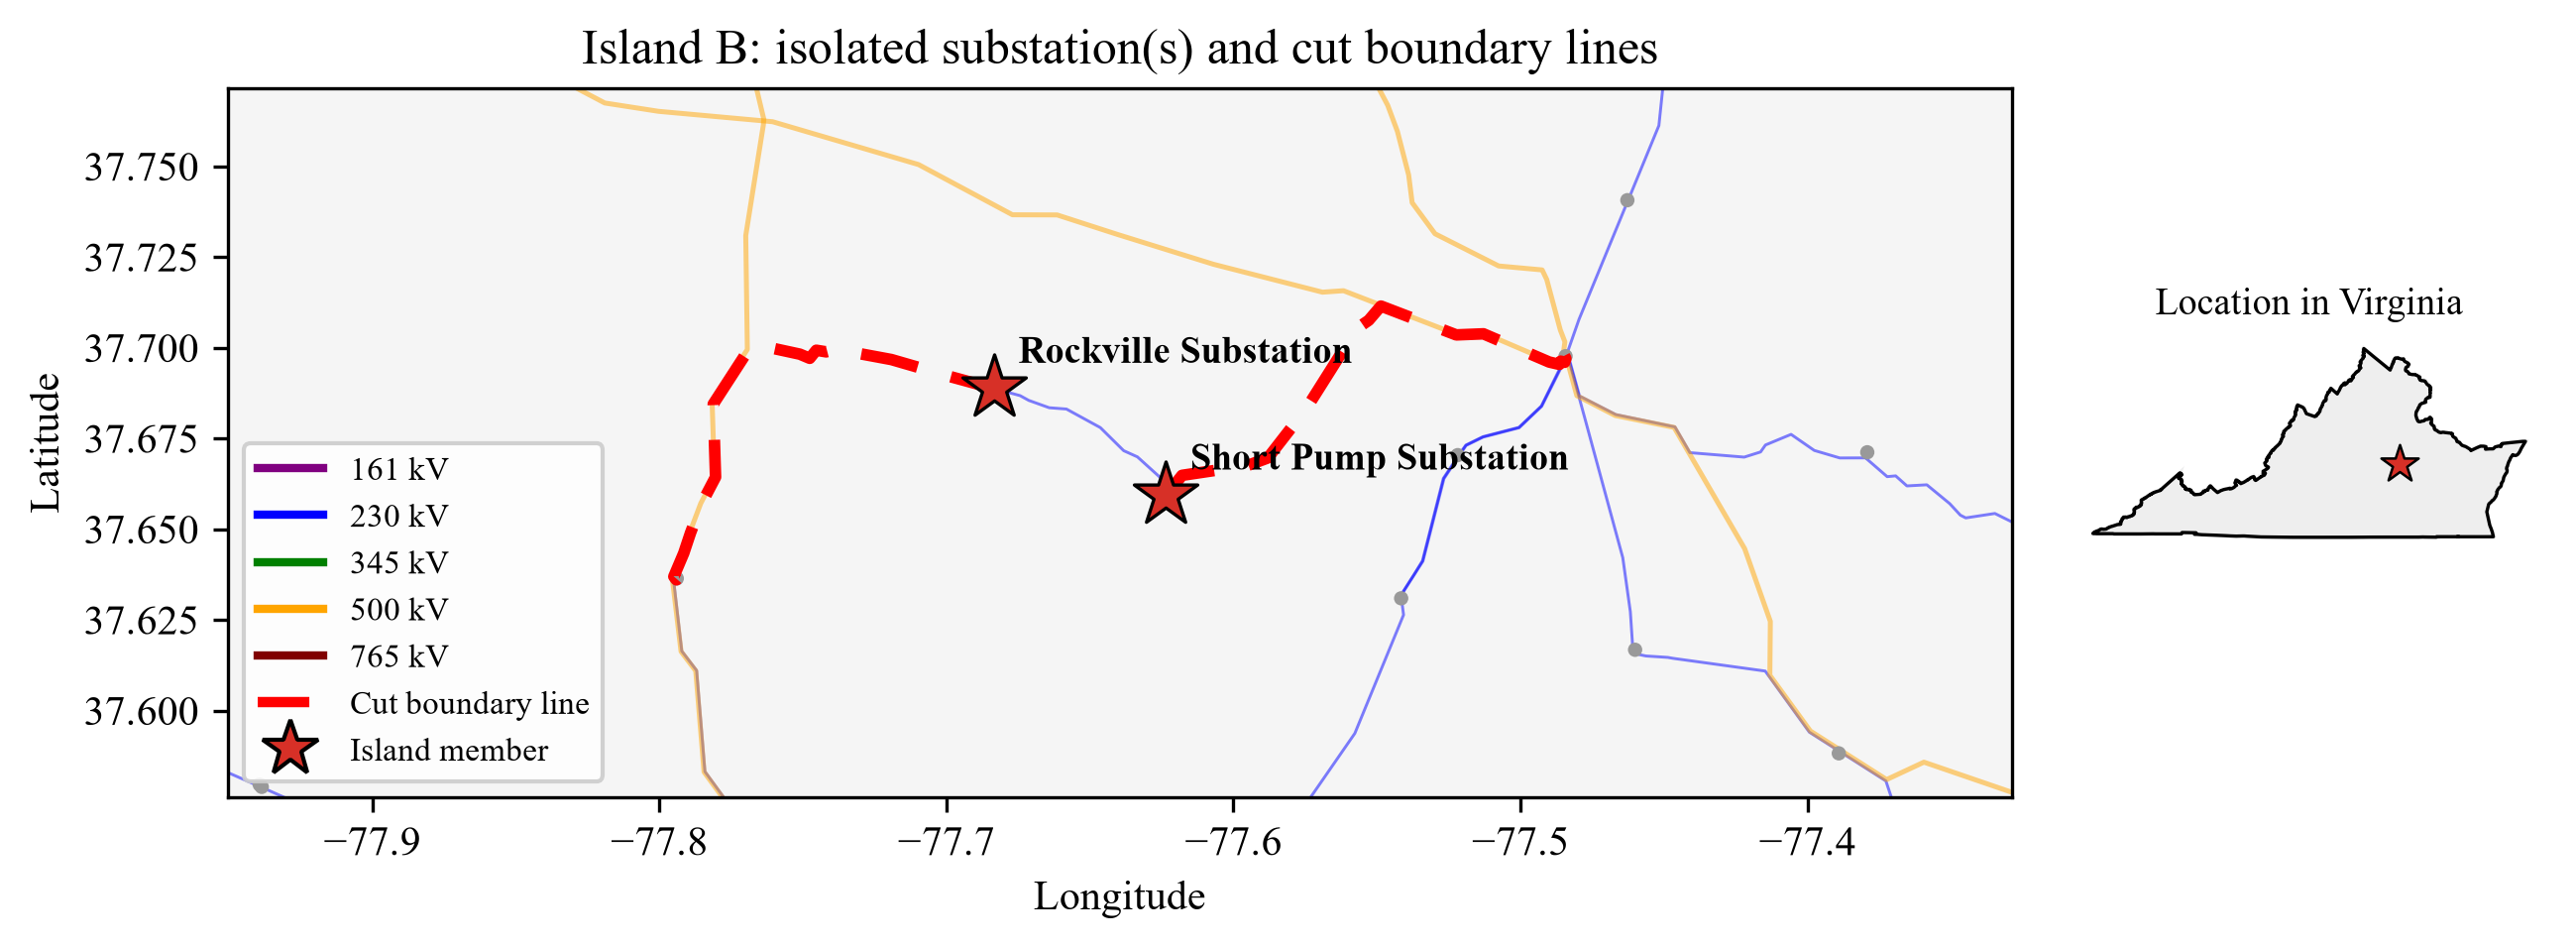
\includegraphics[width=\textwidth]{Figures/va_island_b_map.png}
  \caption{Map of Island B substations and boundary cuts.}
  \label{fig:islandB}
\end{figure}
\begin{figure}[!ht]
  \centering
  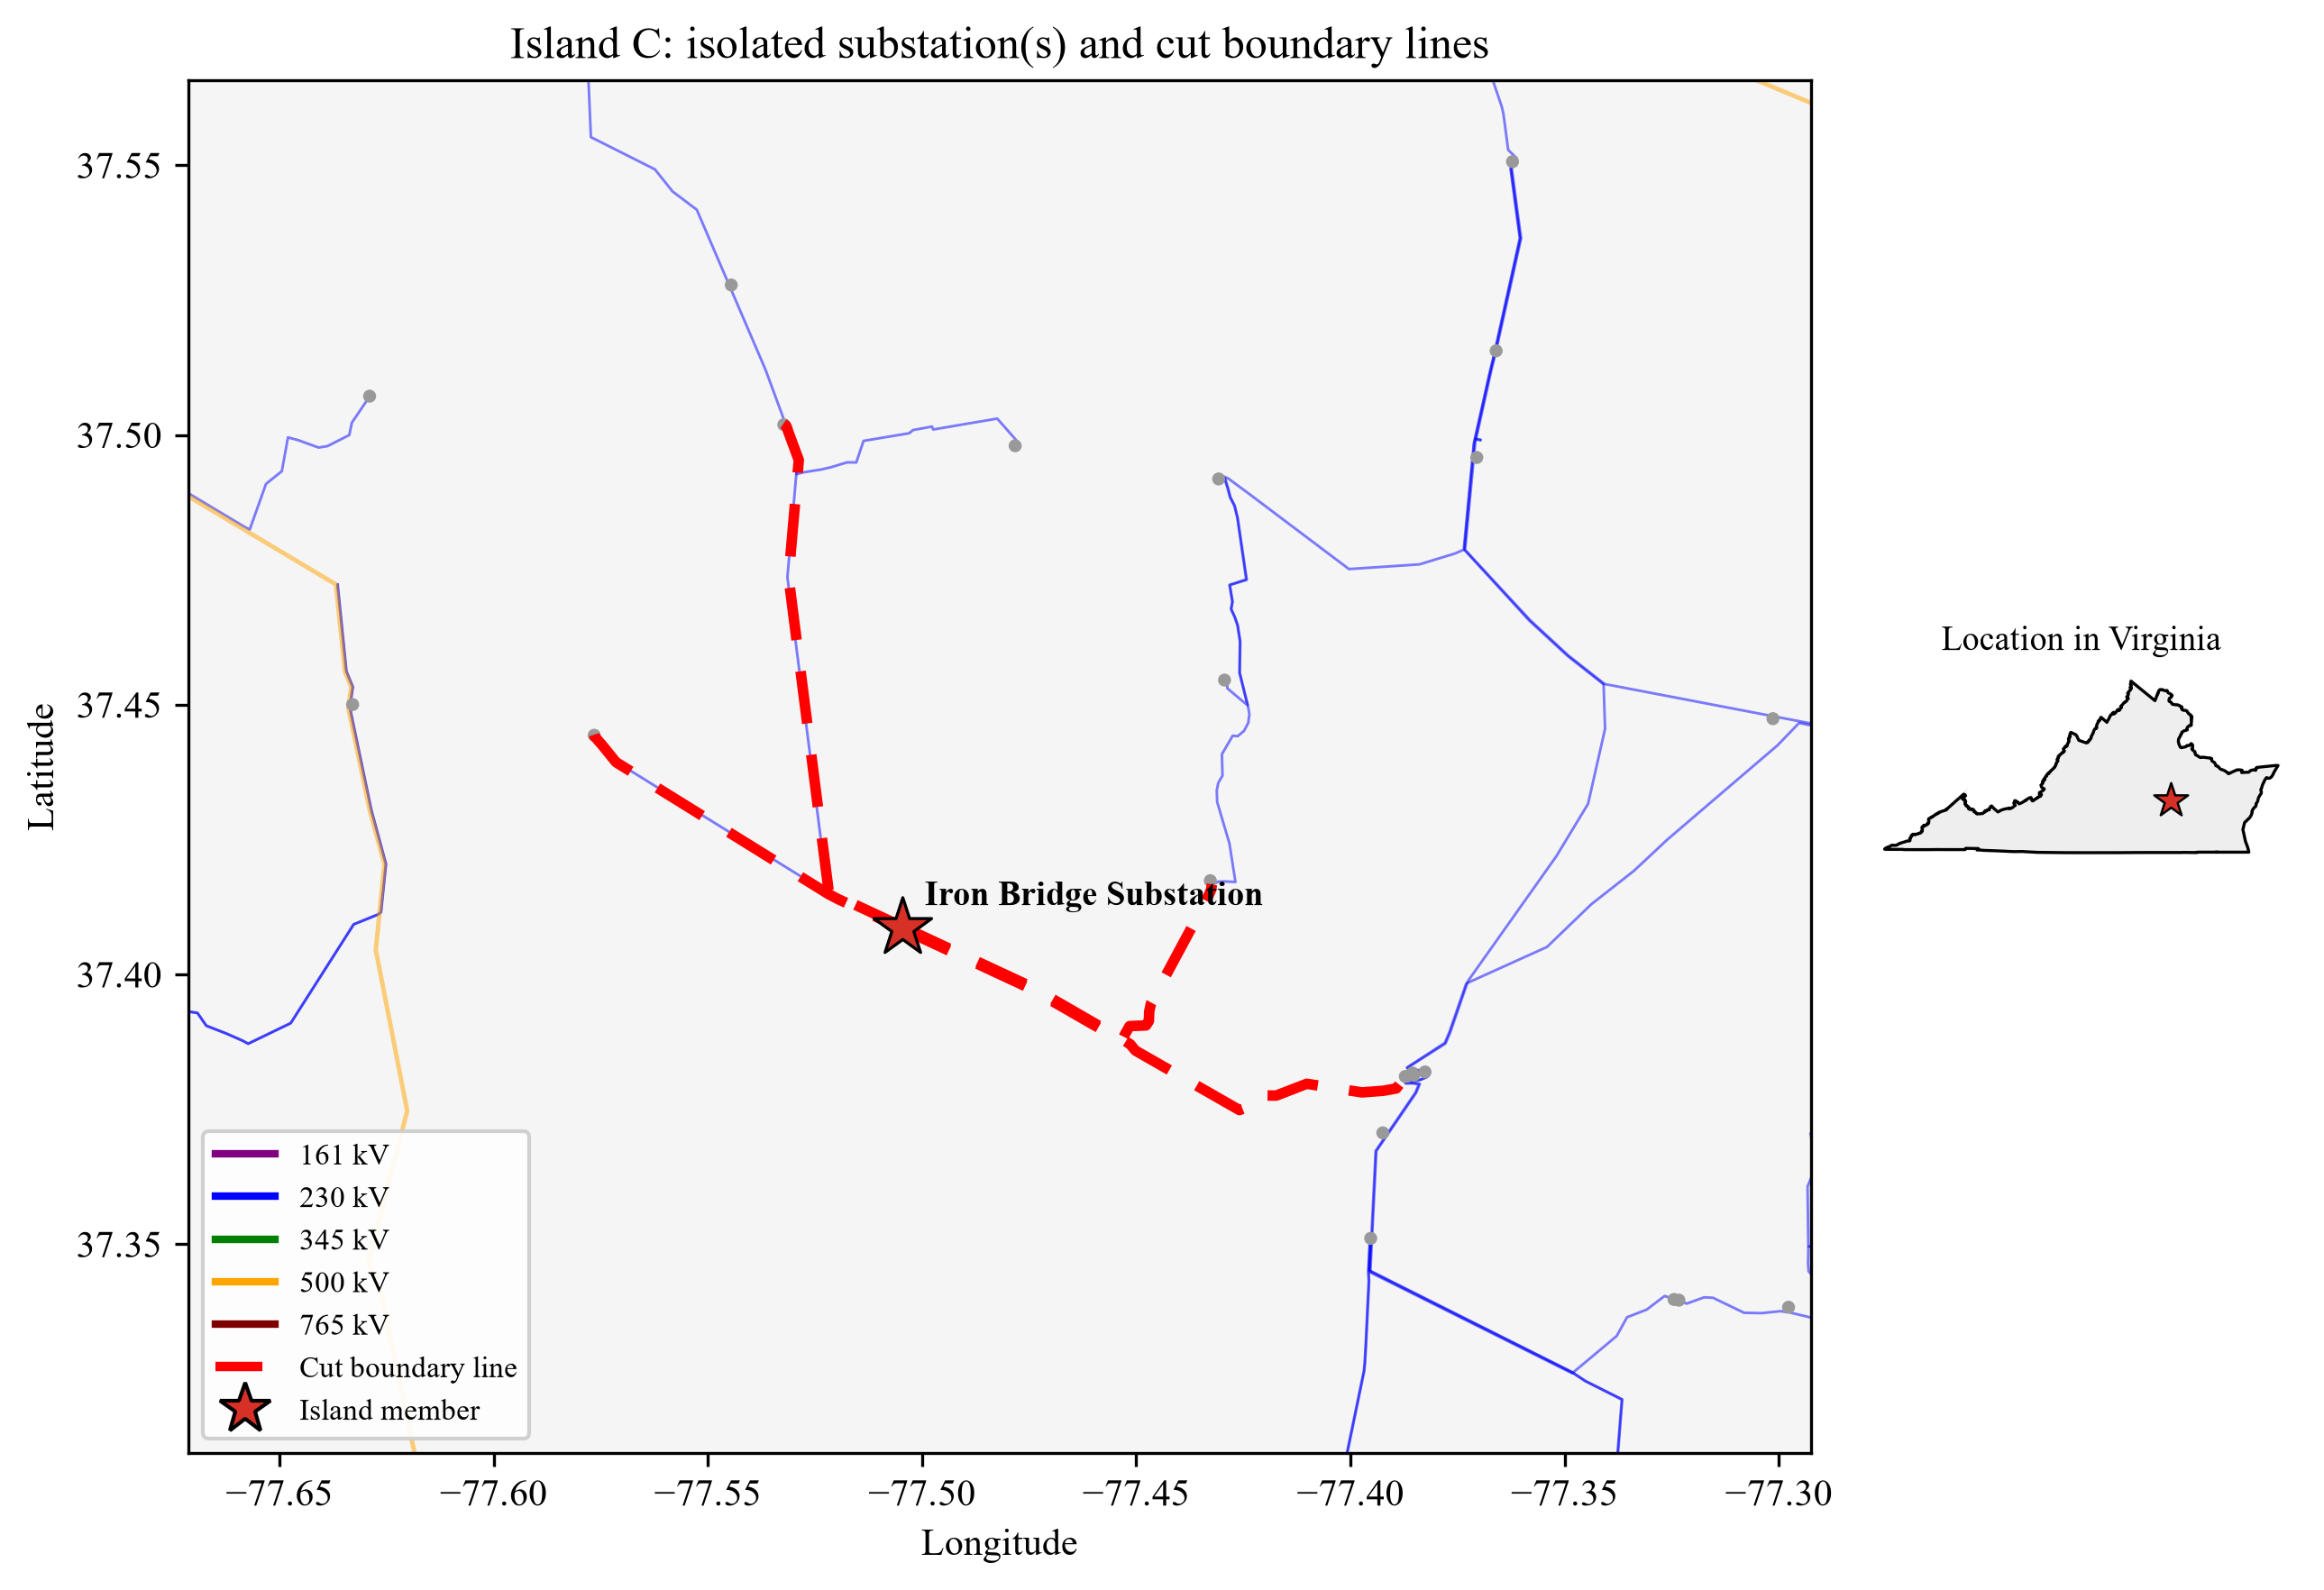
\includegraphics[width=\textwidth]{Figures/va_island_c_map.png}
  \caption{Map of Island C substations and boundary cuts.}
  \label{fig:islandC}
\end{figure}
\clearpage
The three island selection algorithms created Islands A, B, and C, respectively. Island A, outlined in Figure~\ref{fig:islandA}, contains 3 substations: the Winterpock Substation; a substation at $37.45^{\circ}$ N, $77.63^{\circ}$ W; and a substation at $37.25^{\circ}$ N, $77.61^{\circ}$ W. Two transmission lines must be disconnected to make Island A possible. 

Island B, outlined in Figure~\ref{fig:islandB}, contains 2 substations: the Rockville Substation and Short Pump Substation. Two transmission lines must be disconnected to make Island B possible.

Lastly, Island C, outlined in Figure~\ref{fig:islandC}, contains only a single substation, the Iron Bridge Substation. Four transmission lines must be disconnected to make Island C possible. Candidates were rejected if isolating them fragmented the surrounding network, meaning Island C's cut was confirmed not to strand any substation outside the island.

That the search algorithms all found relatively small groups of substations to comprise the islands shows how the greedy formulation favors minimal intervention. Since protective islanding already requires human labor and coordination, the small islands evaluated in this study are likely feasible for a real-world scenario. 


\begin{figure}[!ht]
  \centering
  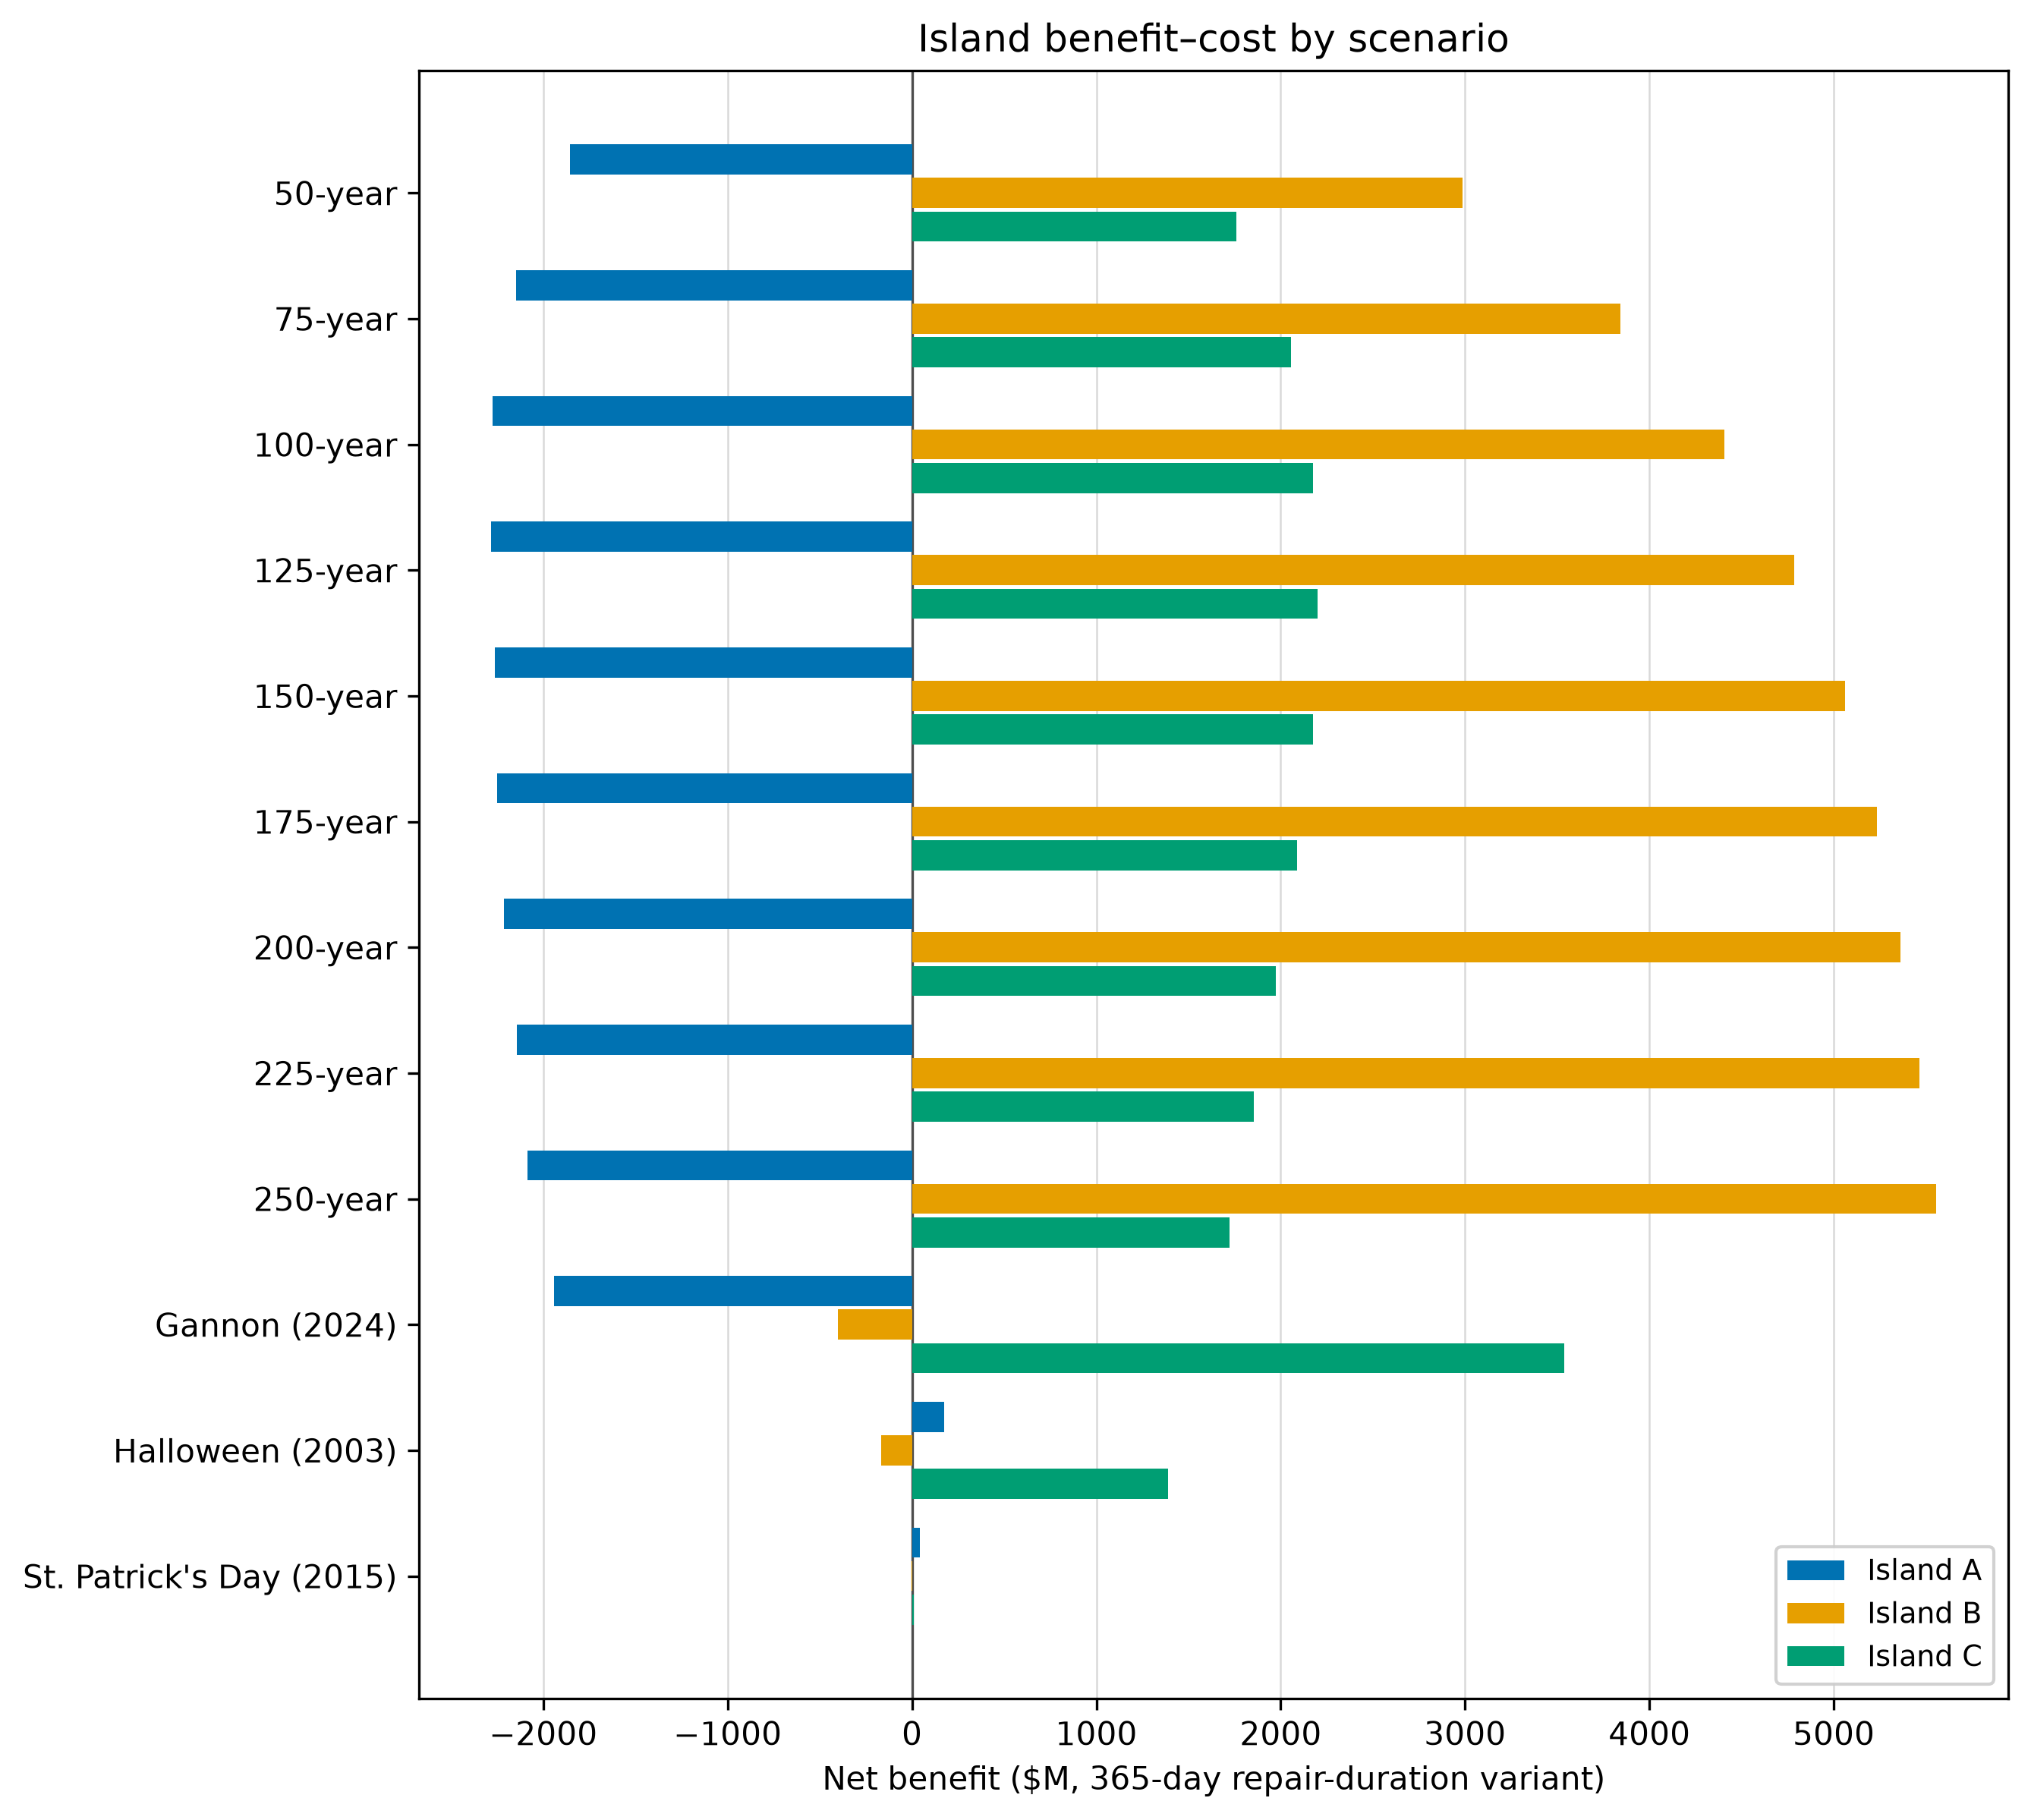
\includegraphics[width=0.95\textwidth]{Figures/va_island_benefit_cost_summary.png}
  \caption{Net benefit by scenario for Islands A, B, and C, assuming 365 days before damaged transformer replacement and a 6-hour disconnection. One-time costs: Island A \$0.1094M (\$0.1000M switching, \$0.0094M outage, two boundary lines); Island B \$0.1129M (\$0.1000M switching, \$0.0129M outage, two boundary lines); Island C \$0.2043M (\$0.2000M switching, \$0.0043M outage, four boundary lines). Full per-scenario benefit, cost, and benefit--cost-ratio values are reported in Tables~S1--S3.}
  \label{fig:islandbenefitcost}
\end{figure}

Economic analysis yielded estimated cost and benefit for each island under the assumption of a 365-day replacement for damaged transformers. Island A, with economic metrics shown in Figure~\ref{fig:islandbenefitcost} (full values in Table~S1), increased economic losses incurred by geomagnetic storms for ten out of twelve evaluated scenarios. This was due to the algorithm settling on an island that caused significant redistribution of GIC to the rest of the network, as evidenced by benefit values below zero. This supports the assertion that considering network-wide distribution following islanding is imperative; creating an island does not guarantee a reduction of GIC impact.

The economic evaluation of Island B (Table~S2) yielded significantly more benefit than cost across all synthetic return periods, as evidence by benefit-cost ratios of tens of thousands to one. At the same time, benefit was negative for all tested historical storms, suggesting a disconnect between Island B's algorithmic selection criteria and the drivers of economic losses for real storms.

The cost-benefit analysis of Island C (Table~S3) showed positive benefit-cost ratios across all twelve tested scenarios. The benefit-cost ratios were typically of a magnitude of several thousand to one, though the benefit-cost ratio was only $\approx50$ in the case of the St. Patrick's Day storm. This suggests that Island C's search algorithm yields islanding that consistently confers economic benefit, though at varying magnitudes.

\section{Conclusion}

This work presents the first state-level adaptation of the U.S. Coupled Space Weather Impact Model (C-SWIM) presented in \citeA{oughton2026majorspaceweatherrisks}. By applying the methodology of the C-SWIM model to the state of Virginia, this work's contributions include a reproducible framework regionally adapting a national physics-engineering-economic pipeline, an actionable assessment of geomagnetic storm risk for Virginia, and a data-driven method of protective islanding evaluated through cost-benefit analysis.

The adaptation framework is a key transferable result of this work. By distingushing between topology-independent factors, such as geomagnetic and geoelectric fields, and topology-dependent factors, such as line voltages, admittance matrices, and induced currents, this work establishes which stages of a national assessment can be subset directly and which require modification. This distinction allows the pipeline to be adapted to any sub-national network without redundant computation or invalid reuse, providing a template for extending coupled space weather risk assessment beyond Virginia.

Adapted to Virginia, the pipeline resolved geomagnetic risk to the level of individual substations, the level at which mitigation can occur. Risk was found to concentrate in central Virginia, particularly the Richmond region, where an elevated geoelectric field coincides with a dense convergence of high-voltage transmission corridors. In measuring economic impact, a 100-year storm was found to cause \$145.5M per day in total losses, rising to \$230.6M per day under a 250-year event, placing between 339,000 and 535,000 people and up to 12,000 businesses at risk. Moreover, Virginia was shown to share a relatively high proportion of geomagnetic storm risk in the United States. These substation-level rankings and regional loss estimates are precisely the information that transmission operators and state energy offices require but national assessments cannot supply.

The exploration of protective islanding for mitigation produced the study's most instructive findings. The algorithm that produced Island A used betweenness centrality and a substation criticality index, proving to worsen economic losses due to betweenness centrality being a poor proxy for islanding importance and a failure to consider network-wide redistribution. Island B's search algorithm proved to be an improvement, incorporating redistribution analysis and current-flow betweenness, but only conferred economic benefit for the synthetic return periods and not historical storms. Only when historical-storm admittance solves were incorporated for Island C's algorithm did islanding confer consistent economic benefit across all twelve tested scenarios, with benefit-cost ratios reaching several thousand to one. This progression demonstrates that protective islanding against geomagnetic storms has considerable economic benefits for a dense, interconnected power grid, but only when network-wide redistribution and storm directionality is considered beyond local or topology-only criteria. 

Several limitations bound these findings. The economic analysis applied a Virginia-localized shock to national social accounting tables; limited public data demanded transformer configurations to be sampled via Monte Carlo; and the pipeline models transformer thermal failure alone, excluding voltage collapse, cascading failure, and restoration, meaning all estimates are conservative lower bounds. The islanding methodology presented in this work depends on assumed disconnection and transformer-replacement durations, which affect the magnitude but not the existence of benefit. Future work includes constructing a region-specific social accounting matrix, applying the adaptation framework to additional regions, and transitioning analysis from protective islanding to resilience islanding, which relies on local generation to prevent even tactical power outages.

\section*{Acknowledgments}\label{acknowledgements}
% [Acknowledgments-P1]
TBD

\section*{Open Research}\label{open-research}
\addcontentsline{toc}{section}{Open Research}

% [Open-Research-P1]
TBD

\section*{Conflict of Interest}
The authors declare there are no conflicts of interest for this manuscript.

\newpage
\bibliography{references}
\end{document}

